\documentclass{gshs_thesis}
\usepackage{graphicx}
\usepackage{multicol}
\usepackage{verbatim}
\usepackage{amsmath, amsfonts, amsthm, amssymb}
\usepackage[utf8]{inputenc}
\usepackage[english]{babel}
\usepackage{hyperref}
\usepackage[capitalize,nameinlink]{cleveref}
\usepackage{spverbatim} 
\usepackage{blindtext}
\usepackage{listings}
\usepackage{xcolor}
\usepackage{kotex}
\hypersetup{
	colorlinks=true,
	linkcolor=black,
	anchorcolor = black,
	citecolor = black,
	filecolor=black,      
	urlcolor=black,
	pdfpagemode=FullScreen
}
\theoremstyle{theorem}
\newtheorem{theorem}{Theorem}[section]
\theoremstyle{lemma}
\newtheorem{lemma}[theorem]{Lemma}
\theoremstyle{definition}
\newtheorem{definition}[theorem]{Defintion}
\lstset{basicstyle=\small\ttfamily,columns=flexible,breaklines=true}
\definecolor{codegreen}{rgb}{0,0.6,0}
\definecolor{codegray}{rgb}{0.5,0.5,0.5}
\definecolor{codepurple}{rgb}{0.58,0,0.82}
\definecolor{backcolour}{rgb}{0.95,0.95,0.92}
\lstdefinestyle{mystyle}{
	backgroundcolor=\color{backcolour},commentstyle=\color{codegreen},
	keywordstyle=\color{magenta},numberstyle=\tiny\color{codegray},
	stringstyle=\color{codepurple},basicstyle=\ttfamily\fontsize{3}{3}\selectfont
	breakatwhitespace=false,breaklines=true,                 
	captionpos=b,keepspaces=true,                 
	numbers=left,numbersep=5pt,                  
	showspaces=false,showstringspaces=false,
	showtabs=false,tabsize=2
}
\lstset{style=mystyle}
\titleheader{졸업논문청구논문}
\school{과학영재학교 경기과학고등학교}
\approval{위 논문은 과학영재학교 경기과학고등학교 졸업논문으로\\
졸업논문심사위원회에서 심사 통과하였음.}
\chairperson{심사위원장}
\examiner{심사위원}
\apprvsign{(인)}
\korabstract{초 록}
\koracknowledgement{감사의 글}
\korresearches{연 구 활 동}
\title{베지어 곡선, 베지어 곡면을 이용한 3D 모델링 개선 연구}
\engtitle{Improvement of 3D Modeling Using Bezier Surface and Bezier Curve}
\korname{박 건 호}
\engname{Park, geonho}
\chnname{朴 建 晧}
\studid{20046}
%------------------------------------------------------------------------
%                  심사위원과 논문 승인 날짜를 입력하시오
%------------------------------------------------------------------------
\advisor{Kim, Soyeon}  %지도교사 영문 이름 (family name, personal name)
\judgeone{박 병 철} %심사위원장
\judgetwo{서 은 아}   %심사위원1
\judgethree{김 소 연} %심사위원2(지도교사)
\degreeyear{2022}   %졸업 년도
\degreedate{2022. 07. 15} %논문 승인 날짜 양식1
\degreedatekor{2022년 07월 15일} %논문 승인 날짜 양식2
%%%%%%%%%%%%%%%%%%%%%%%%%%%%%%%%%%%%%%%%%%%%%%%%%%%%%%%%%%%%%%%%%%%%%%%%%
\checklisttitle{[논문제출 전 체크리스트]}
\checklistI{1. 이 논문은 내가 직접 연구하고 작성한 것이다.}
\checklistmarkI{$\text{\rlap{$\checkmark$}}\square$}
\checklistII{2. 인용한 모든 자료(책, 논문, 인터넷자료 등)의 인용표시를 바르게 하였다.}
\checklistmarkII{$\text{\rlap{$\checkmark$}}\square$}
\checklistIII{3. 인용한 자료의 표현이나 내용을 왜곡하지 않았다.}
\checklistmarkIII{$\text{\rlap{$\checkmark$}}\square$}
\checklistIV{4. 정확한 출처제시 없이 다른 사람의 글이나 아이디어를 가져오지 않았다.}
\checklistmarkIV{$\text{\rlap{$\checkmark$}}\square$}
\checklistV{5. 논문 작성 중 도표나 데이터를 조작(위조 혹은 변조)하지 않았다.}
\checklistmarkV{$\text{\rlap{$\checkmark$}}\square$}
\checklistVI{6. 다른 친구와 같은 내용의 논문을 제출하지 않았다.}
\checklistmarkVI{$\text{\rlap{$\checkmark$}}\square$}
\usepackage{tocloft}
\setlength{\cftbeforesecskip}{0pt}
\setlength{\cftbeforesubsecskip}{0pt}
\setlength{\cftbeforesubsubsecskip}{0pt}
\begin{document}
\baselineskip=2.2em 
\maketitle
\setcounter{page}{1}
\begin{abstracts}  
	\addcontentsline{toc}{section}{Abstract} 
	\noindent{
		Bezier surface and Bezier curve are widely used in the field of designing automobiles and aircraft bodies. The  reason is that it has a very smooth shape and has little memory required for storage. This study deals with new models and RGB storage formats using Bezier surface and Bezier curve for 2D and 3D models. It was created by dividing a model and storing approximate curves and curves, referring to linear studies such as the Möller-Trumbore intersection algorithm, the least squares method, and the Gaussian Newton method. Using this method, the 3D model showed more than 100 times more efficiency than the conventional triangular splitting method, which was often used, and it could be seen with eyes that it became softer than the conventional storage method. This study showed that any model is always approximated enough when using this method. Curve and curved modeling in this study based on mathematical theorical background and programming efficiency are expected to greatly contribute to VR, AR, and hologram fields. In addition, it will be possible to use it more in the CAGD field.
	}
\end{abstracts}
\begin{abstractskor}       
	\addcontentsline{toc}{section}{초록} 
	\noindent{
		Bezier surface, Bezier curve는 자동차의 차체나 비행기의 차체 등을 설계하는 분야에서 많이 사용된다. 그 이유는 Bezier 곡선, 곡면은 매우 매끄러운 형태를 지니며 저장할 때 적은 메모리가 필요하기 때문이다. 이 연구에서는 2D, 3D 모형들에 대해 Bezier surface, Bezier curve를 이용한 새로운 모델 및 RGB 저장형식을 다룬다. 이는 어떤 모형을 분할하여 근사한 곡선, 곡면을 저장하는 형식으로 Möller–Trumbore intersection algorithm, 최소제곱법, 가우스 뉴턴 방법과 같은 선형연구를 참고하여 만들었다. 이 방법을 사용해보면 3D모형은 기존에 많이 사용했던 삼각형 분할 방법보다 100배 이상의 효율을 보였고, 기존의 저장 방법보다 부드러워진 것을 눈으로 확인해볼 수 있었다. 이 방법을 이용할 때 항상 어떤 모형이든 충분히 근사 가능하다는 것을 증명하였다. 이러한 수학적 근거와 프로그래밍 효율성에 기반한 본 연구의 곡선, 곡면 모델링은 VR, AR 및 홀로그램 분야에 크게 기여할 것으로 기대된다. 또한 CAGD 분야에서 더 큰 활용이 가능할 것이다.
	}
\end{abstractskor}
\cleardoublepage
\addcontentsline{toc}{section}{Contents}
\setcounter{secnumdepth}{3} 
\setcounter{tocdepth}{3}
\baselineskip=2.2em
\tableofcontents
\cleardoublepage
\clearpage
\cleardoublepage
\clearpage
\listoffigures
%%%% Main Document %%%%%%%%%%%%%%%%%%%%%%%%%%%%%%%%%%%%%%%%
\cleardoublepage
\clearpage
\renewcommand{\thepage}{\arabic{page}}
\setcounter{page}{1}
\newpage
\section{Introduction}
\subsection{Research motivation}
베지어 곡선과 베지어 곡면을 이용한 연구는 여러 분야에서 이루어지고 있다. 최근에는 베지어 곡선을 이용한 자율 주행 자동차의 경로 탐색에 대한 연구가 있었다.\cite{Ji-wung Choi} 또 베지어 곡선은 흔히 말하는 부드러운 곡선을 만드는 방법을 제시하여 글자 폰트를 만들거나 애니메이션에서 물체의 움직임을 나타내는 데에 사용된다.\cite{Hazewinkel} 이런 베지어 곡선을 이용한 선행 연구에서는 고차 베지어 곡선을 이용한 도형의 근사가 주를 이루었다.\cite{Seon-Hong Kim,Forrest} 베지어 곡면의 경우에는 3D 프린터, 홀로그램 및 VR과 AR 등이 있는데 이러한 기술들이 실제로 상용화되기 위해서는 더 효율적으로 곡면을 다루기 위한 컴퓨터 그래픽 기술이 필요한데 특히 메모리로 인한 처리 시간을 줄이는 기술이 필수적이다. 현재 3D 모델은 저장, 프로그램 사용 등 많은 부분에서 대부분 obj파일 형식으로 사용된다. obj파일에서 곡면을 나타내는 부분을 보면 곡면을 표현하기 위해 삼각형 혹은 사각형 분할을 이용한다는 것을 알 수 있다. 이러한 다각형 분할은 많은 장점이 있지만, 베지어 곡면을 이용한 압축에 비해 구면과 같은 부드러운 곡면을 표현하는 능력이 떨어진다는 단점도 있다. 고차 베지어 곡선, 곡면을 사용하는 선행연구와 달리  본 연구에서는 모델들을 근사할때 베지어 곡선을 2차 베지어 곡선, (2,2)차 베지어 곡면만으로 제한하였다. 그리고 이렇게 제한하므로서 얻는 특징들을 활용하여 곡선을 근사하여 저장하는데 필요한 메모리 용량을 줄일 수 있도록 하였다.  이 과정에서 obj파일 형식으로 주어진 3차원 공간상의 곡면을 조각별로 분할하여 베지어 곡면을 통해 근사 및 압축하는 방법을 제시하였다. 베지어 곡선, 곡면에 움직임을 주는 방법을 3차원으로 확장하여 3차원 곡선, 곡면의 움직임을 줄 수 있음을 보였다.\cite{Bezier Polynomial}  이것은 베지어 곡면 곡선의 고유한 특성 때문에 메모리의 측면에서의 이점을 가진다. 본 연구에서는 \cref{last research}의 후속연구로써 모델 모형 뿐만이 아닌 색상 저장 기법을 개선하는 방법을 제시하고자 한다. 이 방법을 활용하면 기존의 mtl저장 기법에 있는 색깔 반사도 저장 형식을 개선할 수도 있다. 그리고 색상에 대한 저장형식도 개선함으로써 메모리를 압축하는 효과를 기대할 수 있다.
\subsection{Theorectical background}
\subsubsection{베지어 곡선과 곡면, 가중치 베지어 곡선과 곡면}
\begin{definition} \label{BC}
	\textbf{$\boldsymbol{n}$차 베지어 다항식(Bézier polynomial)}은 $n+1$개의 점 $\mathbf{P}_0, \mathbf{P}_1, \cdots, \mathbf{P}_n$에 대해 다음과 같이 주어진다.
	\begin{equation}
		\mathbf{B}:[0,1] \rightarrow \mathbb{R}^{2}, \ \mathbf{B}(t)=\sum_{i=0}^n \binom ni(1-t)^{n-i}t^i\mathbf{P}_i
	\end{equation}
	이때 $n$차 베지어 다항식에 의한 폐구간 $[0, 1]$의 상을 \textbf{$\boldsymbol{n}$차 베지어 곡선(Bézier curve)}이라 한다. 또한 점 $\mathbf{P}_0, \cdots, \mathbf{P}_n$을 이 베지어 곡선의 \textbf{조절점(control point)}이라 한다. 
\end{definition}
\begin{figure}[h]
	\centering
	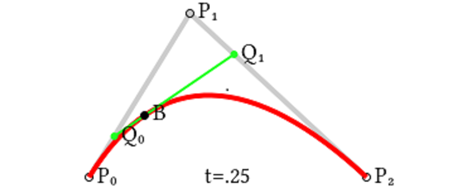
\includegraphics[width=.4\textwidth]{image/BC_model}
	\caption{2차 베지어 곡선}
	\small   
	\raggedright
	곡선의 조절점을 $\textbf{P}_{0},\textbf{P}_{1},\textbf{P}_{2}$라고 할 때 식은 $\textbf{B}(t)=(1-t)^{2}\textbf{P}_{0}+2t(1-t)\textbf{P}_{1}+t^{2}\textbf{P}_{2} \  (t\in{[0,1]})$이다.
\end{figure}
편의상 베지어 곡선을 BC로 표기하자.
\begin{definition} \label{BS}
	$(n+1)(m+1)$개의 점 $\mathbf{b}_{ij}\ (i=0, 1, \cdots, n\ \mathrm{and}\ j=0, 1, \cdots, m)$에 대해 다음 $2$변수 다항식을 생각하자. 
	\begin{equation}\label{BezierSurface}
		\mathbf{x}:[0,1]\times[0,1] \rightarrow \mathbb{R}^{3}, \  \mathbf{x}(u, v)=\sum_{i=0}^n\sum_{j=0}^m B_i^n(u)B_j^m(v)\mathbf{b}_{ij} 
	\end{equation}
	여기서 Bernstein 다항식 $B_i^n(t)=\binom ni(1-t)^{n-i}t^i$로 주어진다. $\mathbf{x}$에 의한 단위 정사각형 $[0, 1]^2$의 상을 \textbf{$\boldsymbol{(n, m)}$-차 베지어 곡면(Bézier surface)}이라 한다. 마찬가지로 점 $\mathbf{b}_{ij}$를 이 베지어 곡면의 조절점이라 한다.\cite{Farin}
\end{definition}
편의상 베지어 곡면을 BS로 표기하자.
\begin{figure}[h]
	\centering
	\begin{subfigure}[b]{.45\textwidth}
		\centering
		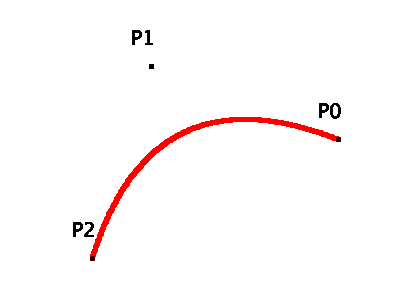
\includegraphics[width=\textwidth]{image/BC}
		\caption{베지어 곡선}
	\end{subfigure}
	\hfill
	\begin{subfigure}[b]{.45\textwidth}
		\centering
		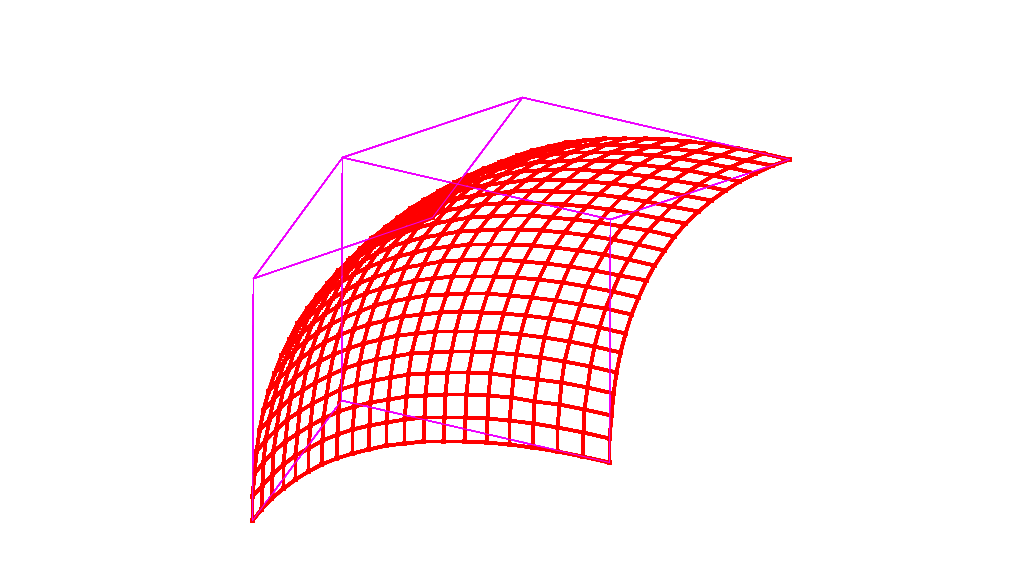
\includegraphics[width=\textwidth]{image/BS}
		\caption{베지어 곡면}
	\end{subfigure}
	\caption{베지어 곡선(a)과 베지어 곡면(b)}
\end{figure}
\begin{definition} \label{WBC}
	\textbf{$\boldsymbol{n}$차 가중치 베지어 다항식(weighted Bézier polynomial)}은 $n+1$개의 점 $\mathbf{P}_0, \mathbf{P}_1, \\  \cdots, \mathbf{P}_n$,  $n+1$개의 RGB 값을 열상에 배열한 색상 벡터 $\mathbf{Q}_0, \mathbf{Q}_1, \cdots, \mathbf{Q}_n$, 위치벡터, 색상벡터를 순서대로 열상에 배열한 색상 조절점 벡터 $\mathbf{K}_0, \mathbf{K}_1, \cdots, \mathbf{K}_n$에 대해 다음과 같이 주어진다.
	\begin{equation}
		\begin{split}
		   \mathbf{B}(t)=\sum_{i=0}^n \binom ni(1-t)^{n-i}t^i\mathbf{P}_i  \\
		    \mathbf{C}(t)=\sum_{i=0}^n \binom ni(1-t)^{n-i}t^i\mathbf{Q}_i  \\
		    \mathbf{F}(t)=\sum_{i=0}^n \binom ni(1-t)^{n-i}t^i\mathbf{K}_i
		\end{split}		
    	\label{eq003}
	\end{equation}
	이때 $n$차 베지어 다항식에 의한 폐구간 $[0, 1]$의 점 $\mathbf{B}(t)$에 $\mathbf{C}(t)$ 색상을 입힌 상을 \textbf{$\boldsymbol{n}$차 가중치베지어 곡선(Bézier curve)}이라 한다. 또한 점 $\mathbf{P}_0, \cdots, \mathbf{P}_n$을 이 가중치 베지어 곡선의 \textbf{조절점(control point)}이라 한다. $\mathbf{K}_0, \cdots, \mathbf{K}_n$을 이 가중치 베지어 곡선의 \textbf{RGB 조절점(RGB control point)}이라 한다.
\end{definition}
편의상 가중치 베지어 곡선을 WBC로 표기하자.
\begin{definition} \label{WBS}
	$(n+1)(m+1)$개의 점 $\mathbf{b}_{ij}\ , (n+1)(m+1)$개의 색상벡터 $\mathbf{q}_{ij}\ (i=0, 1, \cdots, n\ \mathrm{and}\ j=0, 1, \cdots, m)$ 색상 조절점 벡터 $\mathbf{k}_{ij}\ (i=0, 1, \cdots, n\ \mathrm{and}\ j=0, 1, \cdots, m)$에 대해 다음 $2$변수 다항식을 생각하자. 
	\begin{equation}
		\begin{split}
		\mathbf{x}(u, v)=\sum_{i=0}^n\sum_{j=0}^m B_i^n(u)B_j^m(v)\mathbf{b}_{ij}  \\  
		\mathbf{c}(u, v)=\sum_{i=0}^n\sum_{j=0}^m B_i^n(u)B_j^m(v)\mathbf{q}_{ij}  \\
		\mathbf{f}(u, v)=\sum_{i=0}^n\sum_{j=0}^m B_i^n(u)B_j^m(v)\mathbf{k}_{ij}
		\end{split}
	  \label{eq004}
	\end{equation}
	여기서 Bernstein 다항식 $B_i^n(t)=\binom ni(1-t)^{n-i}t^i$로 주어진다. $\mathbf{x}$에 $\mathbf{c}$ 색상을 입힌 단위 정사각형 $[0, 1]^2$의 상을 \textbf{$\boldsymbol{(n, m)}$-차 가중치 베지어 곡면(weighted Bézier surface)}이라 한다. 마찬가지로 점 $\mathbf{b}_{ij}$를 이 베지어 곡면의 조절점, $\mathbf{k}_{ij}$를 이 베지어 곡면의 RGB 조절점이라 한다.
\end{definition}
편의상 가중치 베지어 곡면을 WBS로 표기하자.
\begin{figure}[h]
	\centering
	\begin{subfigure}[b]{.45\textwidth}
		\centering
		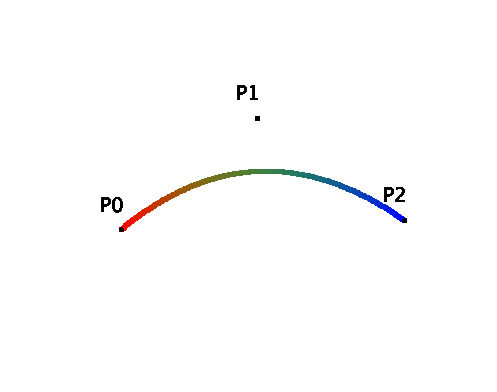
\includegraphics[width=\textwidth]{image/WBC}
		\caption{가중치 베지어 곡선}
	\end{subfigure}
	\hfill
	\begin{subfigure}[b]{.45\textwidth}
		\centering
		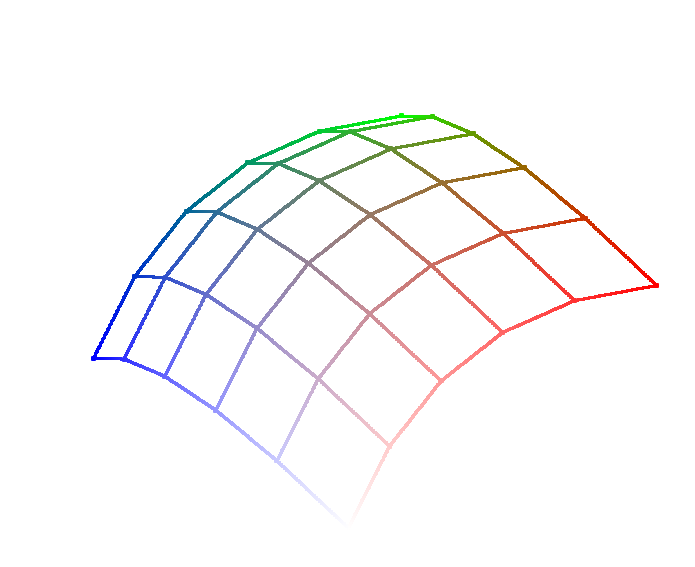
\includegraphics[width=\textwidth]{image/WBS}
		\caption{가중치 베지어 곡면}
	\end{subfigure}
	\caption{가중치 베지어 곡선(a)과 가중치 베지어 곡면(b)}
\end{figure}
\subsubsection{근사 기법}
\begin{definition}
\textbf{뉴턴-랩슨 방법(Newton–Raphson method)}은 미분가능한 실수값 함수의 근을 찾는 알고리즘이다. 미분가능한 함수 $f\colon(a, b)\to\mathbb{R}$과 도함수 $f^\prime$에 대해, 현재 $f(x)=0$의 해의 근사치를 $x_n$이라 하자.  $f$의 선형 근사는 다음과 같다.
\begin{equation*}
	y=f^\prime(x_n)(x-x_n)+f(x_n)
\end{equation*}
다음 근사치 $x_{n+1}$은 위 직선의 $x$절편으로 주어진다.
\begin{equation} \label{newton}
	x_{n+1}=x_n-\frac{f(x_{n})}{f^\prime(x_n)}
\end{equation}
초기값 $x_0$부터 시작해 \cref{newton}을 반복해 더 좋은 근사치를 얻을 수 있다. 그러나 초기값의 선택에 따라 $\{x_n\}$이 발산할 수 있다. 그리고 $f$가 근을 가지지 않는다면 국소 최솟값을 얻는다.
\end{definition}
\begin{definition}
\textbf{가우스-뉴턴 방법(Gauss-Newton Method)}은 뉴턴-랩슨 방법을 다변수 벡터함수로 확장한 것이다. 함수 $\mathbf{f} \colon \mathbb{R}^n \to \mathbb{R}^m$에 대해 $\mathbf{f}(\mathbf{x}) = \mathbf{0}$의 해의 근사치를 $\mathbf{x}_n$이라 하자. 뉴턴-랩슨 방법과 비슷하게 $\mathbf{x}_n$에서 $\mathbf{f}$의 선형 근사를 구한다. 
$$ \mathbf{f}(\mathbf{x}) \approx \mathbf{f}(\mathbf{x}_n) + \mathbf{J}_{\mathbf{f}}(\mathbf{x}_n) (\mathbf{x} - \mathbf{x}_n) $$
이때 $\mathbf{f}$의 \textbf{야코비 행렬(Jacobian matrix)} $\mathbf{J}_{\mathbf{f}}$는 다음과 같은 $m \times n$ 행렬이다. 
$$ \mathbf{J}_{\mathbf{f}}= \begin{pmatrix} \partial f_1 / \partial x_1 & \partial f_1 / \partial x_2 & \cdots & \partial f_1 / \partial x_n \\ \partial f_2 / \partial x_1 & \partial f_2 / \partial x_2 & \cdots & \partial f_2 / \partial x_n \\ \vdots & \vdots & \ddots & \vdots \\ \partial f_m / \partial x_1 & \partial f_m / \partial x_2 & \cdots & \partial f_m / \partial x_n \end{pmatrix}$$

$\mathbf{f}(\mathbf{x}_{n+1}) = \mathbf{0}$이라 하면 $\mathbf{J}_{\mathbf{f}}(\mathbf{x}_n) (\mathbf{x}_{n+1} - \mathbf{x}_n) = -\mathbf{f}(\mathbf{x}_n)$이고, 양변에 $\mathbf{J}_\mathbf{f}$의 의사역행렬(pesudo-inverse)를 곱해 다음 해의 근사치를 얻는다. 
$$ \mathbf{x}_{n+1} = \mathbf{x}_n - (\mathbf{J}_{\mathbf{f}}(\mathbf{x}_n)^\intercal \mathbf{J}_{\mathbf{f}}(\mathbf{x}_n))^{-1} \mathbf{J}_{\mathbf{f}}(\mathbf{x}_n)^\intercal \mathbf{f}(\mathbf{x}_n) $$
실제로 $m = n = 1$이라면 이는 뉴턴-랩슨 방법과 같다.
\end{definition}
\subsubsection{경계 (Boundary)}
\begin{definition}
	위상공간 $(X, \mathfrak{I})$의 부분집합 $A$의 \textbf{내부(interior)}와 \textbf{폐포(closure)}, \textbf{경계(boundary)}는 각각 다음과 같이 정의된다 \cite{Munkres.J.}.
	\begin{align*}
		A^\circ &= \bigcup \{ U \subset A \mid U \in \mathfrak{I} \} \\
		\bar{A} &= \bigcap \{ C \supset A \mid X-C \in \mathfrak{I} \} \\
		\partial A &= \bar{A} - A^\circ
	\end{align*}
   특히 $\bar{A}$는 A의 원소와 A의 극한점(limit point)로 이루어진다.
\end{definition}
\subsubsection{볼록집합 (Convex set)}
\begin{definition}
	$\mathbb{R}^n$의 부분집합 $C$가 다음 조건을 만족할 때, $C$를 \textbf{볼록 집합(convex set)}이라 부른다. 
	\begin{equation*}
		\forall \mathbf{x}, \mathbf{y} \in C,\ \forall t \in [0, 1],\ (1-t)\mathbf{x}+t\mathbf{y} \in C
	\end{equation*}
    \begin{lemma} \label{closureofconvexset}
	$C \subset \mathbb{R}^n$가 볼록집합이면, $C$의 폐포(closure) $\bar{C}$도 볼록집합이다. 
    \end{lemma}
    \begin{proof}
	임의의 $\mathbf{x}, \mathbf{y} \in \bar{C}$와 $t \in [0, 1]$에 대해 $(1-t)\mathbf{x} + t\mathbf{y} \in \bar{C}$임을 보이자. $\mathbf{x}, \mathbf{y} \in \bar{C}$이므로 적당한 수열 $\{ \mathbf{x}_n \}, \{ \mathbf{y}_n \} \subset C$이 존재해 $\mathbf{x}_n \to \mathbf{x}, \, \mathbf{y}_n \to \mathbf{y}$를 만족한다. 각 자연수 $n$에 대해 $\mathbf{x}_n$과 $\mathbf{y}_n$은 볼록집합 $C$의 원소이므로 $(1-t)\mathbf{x}_n + t\mathbf{y}_n \in C$이다. 이제 $n \to \infty$의 극한을 취하면 $(1-t)\mathbf{x} + t\mathbf{y} \in \bar{C}$를 얻는다. 
    \end{proof}
    \begin{theorem} \label{homeo}
	$\mathbb{R}^n$의 볼록 집합 $C$의 내부(interior)가 공집합이 아닐 때, $C$의 경계(boundary) $\partial C$는 $S^{n-1}$과 위상동형이다. 여기서 $S^{n-1}$은 $(n-1)$차원 단위 구면으로, $S^{n-1}=\{ \mathbf{x}\in\mathbb{R}^n \mid \| \mathbf{x} \| = 1 \}$이다.
    \end{theorem}
간단히 증명하면, $C$의 내부가 공집합이 아니므로 $C$를 평행이동하여 $\mathbf{0}\in C^\circ$가 되도록 만들 수 있다. 이제 함수 $f\colon\partial C \to S^{n-1}$을 $\phi(\mathbf{x})=\mathbf{x}/\|\mathbf{x}\|$로 정의하면 $\phi$는 위상동형사상이 된다. 
\end{definition}
\subsubsection{오차함수}
우리는 2D 인지, \ 3D인지 모델만 근사를 하는건지, \ 색상까지 근사를 하는건지에 따라 적절한 오차함수를 상황에 따라 고를 필요가 있다. 2가지 오차함수를 정의하여 상황에 따라 이를 그대로 또는 변형해서 사용할 것이다. 
\begin{definition}
	거리공간 $(M, d)$의 공집합이 아닌 두 부분집합 $X, Y$에 대해 하우스도르프 거리는 다음과 같이 주어진다. \cite{Munkres.J.}
	\begin{equation} \label{hausdorffdistance}
		d_H(X, Y) = \max \left\{ \sup_{x \in X} \inf_{y \in Y} d(x, y), \, \sup_{y \in Y} \inf_{x \in X} d(x, y) \right\}
	\end{equation}
\end{definition}
하우스도르프 거리는 거리공간 상에서 두 집합이 서로 떨어진 정도를 나타낸다. 실제로, $d_H(X, Y) = 0$일 필요충분조건은 $X$와 $Y$의 폐포가 일치하는 것이다. 
\begin{definition}
	모델 부분에서 오차함수는 다음과 같이 정의한다. 분할된 각 영역 내의 점을 $\mathbf{P}_k\ (1\leq k\leq K)$라 하고, 이에 대응되는 베지어 곡면 위의 점을 $\mathbf{x}(u_k, v_k)=\mathbf{x}_k$라 하자. 이때 오차함수 $\mu$는 다음과 같이 주어진다.
	\begin{equation} \label{error2}
		\mu=\max_{\text{각 영역}}\max_{1\leq k\leq K} \| \mathbf{x}_k-\mathbf{P}_k \|
	\end{equation}
\end{definition}
\subsubsection{obj,mtl파일}
obj는 3D 이미지를 저장하는 표준적인 파일이다. obj 파일은 정점 $v$, 단위 법선벡터 $v_n$, 텍스쳐 $v_t$, 면 $F$로 이루어진다. 먼저 $v, v_n, v_t$의 $x, y, z$성분이 차례로 주어진다. 마지막에 $F$가 주어지는데, 각각의 $F$는 $v / v_n / v_t$ 블록 3개 또는 4개로 이루어진다. 3개면 삼각형 면, 4개면 사각형 면이다. 

앞으로 obj파일의 정점 $v$를 $\mathbf{P}_k$로 나타낸다. 그리고 obj파일로 주어진 곡면은 면 $F$들의 합집합을 의미한다.
\begin{verbatim}
	# object heart
	
	v -5.7868 -2.8897 6.9550
	v -5.8939 -2.7443 6.7745
	...
	v 1.3498 1.7948 1.8726
	# 5636 vertices
	
	vn -0.3934 -0.8264 -0.4029
	...
	vn 0.2663 0.7947 -0.5454
	# 5634 vertex normals
	
	vt 0.1020 0.1559 0.0000
	...
	vt 0.7205 0.0233 0.0000
	# 5974 texture coordinates
	
	g Heart       # o [object name] / g [group name] 
	usemtl Heart  # usemtl [material name]
	s 1           # s : smooth
	f 1/1/1 2/2991/2 3/1583/3 4/2994/4
	...
	f 5598/1580/5598 5595/5955/5595 5634/2990/5634 5633/5974/5633
\end{verbatim} 
mtl은 ambient 반사도 $K_a$, diffuse 반사도 $K_d$, specular 반사도 $K_s$ 등으로 이루어진다. 모두 0에서 1 사이의 값을 가지며 각각 물체가 원래 가지고 있는 색에 의한 반사도, 국소적인 색에 의한 반사도, 하이라이트를 일으키는 반사도를 의미한다. 본 연구에서는 $K_a$ 및 $K_d$만 사용했다. 

\subsection{연구질문}
본 연구에서의 연구 질문은 다음과 같다. 
\begin{enumerate}
	\item 구간을 어떻게 나눌것인가?
	\item 모델들이 베지어 곡선, 베지어 곡면을 이용해 점들을 충분히 근사할 수 있다. (i.e. 오차함수가 0으로 수렴한다)
	\item obj 등 기존의 곡면을 저장하는 방식보다 더 높은 압축 효율을 가진다.
	\item 기존 mtl과 같이 곡면이 지닌 색, 질감 등의 성질도 베지어 곡면의 특징을 이용해 압축하여 저장할 수 있다.
	\item 근사하거나 구현하는 과정에서 시간이 obj저장 기법보다 적게 소모된다.
	\item 각 방법마다 새로 정의한 오차함수가 적절한가?
	\item 색상이 있어도 충분히 근사 가능하다. 
\end{enumerate}
\section{Main Contents}
우리는 어떠한 모델들을 근사하여 메모리를 압축하는 방법들을 다룰 것이다. 일단 기존의 삼각형 분할처럼 베지어 곡면으로도 저장이 가능하다고 보여야한다. 어떠한 모델을 가져다 놓더라도 일단 (2,2)차 베지어 곡면 하나로는 안된다는 건 스파이크 모형만 제시하여도 튀어나온 부분이 다 근사가 되지 않으므로 알 수 있다. 그러면 우리는 곡면의 차원을 높이거나 그 곡면을 여러개 둠으로서 해결할 수 있다. 이 연구에서는 지금까지의 많은 선행연구와 달리 삼각형을 많이 두는 잇는 것처럼 (2,2)차 베지어 곡면을 많이 둘 것이다. 이것은 결국 (2,2)차 베지어 곡면을 두는 방법과 하나의 베지어 곡면을 결정하게 되는 영역의 분할하는 방법을 알아야 함을 의미한다. 그리고 이를 근사하면 이게 알맞게 근사되었는지 알 수 있도록 오차함수를 잡아야 하는데 이를 잘 설정해야 잘 근사되었다고 할 수 있을 것이다. 

이 연구에서는 2차원 물체와 3차원 물체를 근사해볼 것이다. 그리고 각각에 대해 바로 색상으로 확장하기에는 무리가 있어 단색 모델이 있을때 이를 근사해보는 것을 먼저 알아볼 것이다. 

각각의 근사에 대해서 알아볼때 분할하는 방법 그리고 분할 했을때 곡면을 정의해야하므로 조절점을 결정하는 방법, 그리고 각각에 적절한 오차함수를 제시하고 적절성을 설명할 것이다. 
\subsection{2D Model Improvement}
먼저 우리는 2D 단색 모델에 대한 근사 방법을 알아볼 것이다. 
\subsubsection{분할 방법}
분할하는 방법을 정의하기 위해서는 조각이랑 조각별이라는 개념을 사용할 필요가 있다.그리고 분할함에 있어서 오차함수도 새로 정의할 필요가 있다.
\begin{definition}
   곡선  $C$가 연속함수 $\gamma:[a:b]\rightarrow\mathbb{R}^{3}$ 의 상 $\gamma([a,b])$로 정의된다고 하자. $a=x_{0}<x_{1}<\cdots<x_{n}=b$인 ${\{x_i\}}^{n}_{i=0}$에 대해 $\gamma$의 정의역을 $[{x}_{i-1},{x}_{i}]$로 축소시킨 $n$개의 함수 ${\{{\gamma_{i}\}}^{n}_{i=1}}$로 나누는 것을 \textbf{조각별}로 나눈다고 한다. 또한 각각의 $\gamma_{i}$에 의한 의 $[{x}_{i-1},{x}_{i}]$상을 곡선의 \textbf{조각}이라 한다. 
   \begin{figure}[h]
   	\centering
   	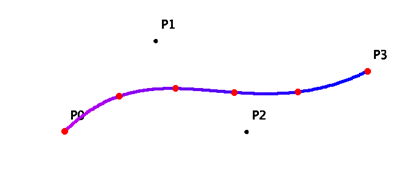
\includegraphics[width=.5\textwidth]{image/piece}
   	\caption{조각별과 조각}
   	\small 빨간 점을 기준으로 곡선을 조각별로 나누는 그림, 나누어진 각각의 곡선을 조각이라 한다.
   \end{figure}
\end{definition}
\begin{definition}
    곡선 $C$를 $\{C_{i}|i\in{I}\}$와 같이 조각별로 나누었다고 하자. 각 $i\in{I}$에 대해 $C_{i}$를 근사한 곡선을 $B_{i}$라 하면 \textbf{근사 거리}는 다음과 같이 주어진다.
     \begin{equation}
     	\mu_{i}=d_{H}(C_{i},B_{i})
     \end{equation}
   전체 곡선 $C$와  $B=\cup_{i\in{I}}B_{i}$사이의 \textbf{근사 거리}는 다음과 같다.
     \begin{equation}
   	    \mu=\max_{i\in{I}}\mu_{i}
     \end{equation}
\end{definition}
\begin{definition}
	곡선 $C$와  $B$사이의 근사 거리를 $\mu$라 하자. 임의의 $\epsilon>0$에 대해 $\mu<\epsilon$이 성립하면 $B$는 $C$에 \textbf{충분한 근사}가 됐다고 하자.
\end{definition}
이제 우리는 어떤 영역 사이의 점이 주어졌을때 분할하는 방법과 이에 대한 오차함수를 알아보았다. 2D 모델 근사에서의 점은 선적분으로 얻은 길이의 절반이 되는 점으로 한다. 
\subsubsection{Control Point Determination}
어떤 2D 모델을 근사하기 위해서 우리는 분할하는 방법을 다루었다. 그러면 우리는 분할한 영역에 대해서 하나의 베지어 곡선으로 근사시킬것이기 때문에 조절점 3개를 정해야한다. 양끝점은 분할한 영역의 끝점으로 하면 우리는 중간 조절점을 찾는 문제만 남는다. 이 조절점을 찾는 과정은 다음 정리를 이용하여 해결한다.
\begin{theorem}\label{BCmiddle}
	서로 다른 세 점 $\textbf{P}_{0},\textbf{P}_{1},\textbf{P}_{2}$를 조절점으로 가지는 2차 베지어 곡선에 대해 곡선 위의 한 점에서 $\textbf{P}_{0}$과 $\textbf{P}_{2}$를 잇는 직선에 내린 수선의 길이가 최대가 되는 점을 $\textbf{Q}$라 하면 $\textbf{Q}=(\textbf{P}_{0}+2\textbf{P}_{1}+\textbf{P}_{2})/4$이다.
\end{theorem}
\begin{proof}
		우선 2차 베지어 곡선은 다음과 같이 주어진다. 
		\begin{align*}
			\mathbf{B}(t) &= (1-t)^2 \mathbf{P}_0 + 2t(1-t) \mathbf{P}_1 + t^2 \mathbf{P}_2 \\
			&= (1-t)((1-t)\mathbf{P}_0 + t\mathbf{P}_1) + t((1-t)\mathbf{P}_1 + t\mathbf{P}_2)
		\end{align*}
		세 점 $\mathbf{P}_0, \mathbf{P}_1, \mathbf{P}_2$는 하나의 평면 $\alpha$를 결정한다. $(1-t)\mathbf{P}_0 + t\mathbf{P}_1$과 $(1-t)\mathbf{P}_1 + t \mathbf{P}_2$는 각각 $\mathbf{P}_0$와 $\mathbf{P}_1$, $\mathbf{P}_1$과 $\mathbf{P}_2$의 $t \colon (1-t)$ 내분점이므로 $\alpha$ 위에 있다. 또한 $\mathbf{B}(t)$도 $\alpha$ 위에 있고, 따라서 2차 베지어 곡선은 하나의 평면에 놓여있다. 
		
		이 평면 위에서 다음을 만족하는 직교좌표계 $(x^\prime, y^\prime)$를 만들 수 있다.
		$$ \mathbf{P}_0 = \begin{pmatrix} -a \\ 0 \end{pmatrix}, \quad \mathbf{P}_1 = \begin{pmatrix} b \\ c \end{pmatrix}, \quad \mathbf{P}_2 = \begin{pmatrix} a \\ 0 \end{pmatrix}, \quad (a, b, c > 0) $$
		그러면 $\mathbf{Q}$는 $y^\prime$좌표가 최대인 점이다. $\mathbf{B}(t)$의 $y^\prime$좌표는 $2ct(1-t)$이므로, $t = 1/2$일 때 최대이다. $\mathbf{Q} = \mathbf{B}(1/2) = (b/2, \, c/2)^\intercal$이므로 위 정리가 성립한다. 
\end{proof}
\begin{figure}[h]
	\centering
	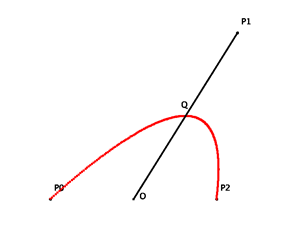
\includegraphics[width=.5\textwidth]{image/BCmiddle}
	\caption{2차 베지어 곡선의 성질}
	\raggedright \small 베지어 곡선 위의 한 점에서 $\textbf{P}_{0}$과 $\textbf{P}_{2}$를 잇는 직선에 내린 수선의 길이가 최대가 되는 점을 $\textbf{Q}$라 하면 $\textbf{Q}=(\textbf{P}_{0}+2\textbf{P}_{1}+\textbf{P}_{2})/4$로 주어진다.
\end{figure}
이 연구에서는 위의 방법으로 중간 조절점을 잡는다. 
\subsubsection{Algorithm} \label{arc_approxiamtion}
지금까지 분할방법과 중간 조절점을 정하는 방법으로 실제로 원호를 근사해볼 것이다.
위에서 우리는 오차함수를 새로 정의하였는데 어떤 기준값을 설정하여 그 기준값보다 오차함수가 작으면 그대로 종료 아니면 위에서 소개한 분할 방법인 선적분한 길이의 중간 점을 잡아 구간을 분할하고 각각의 조각을 베지어 곡선으로 근사시킬 것이다. 그리고 오차함수가 기준값에서 작아질때까지 계속 반복할 것이다.

일단 조각별로 나누는 과정을 시각적으로 확인해보자
연속함수 $\gamma:[0,1]\rightarrow\mathbb{R}^{3}$에 대해 $C=\mathbb{\gamma}([0,1])$이라 하자. $n\in\mathbb{N}$에 대해 곡선을 다음과 같이 $2^{n}$개의 조각으로 나눈다.
\begin{equation}
	\begin{split}
		&\gamma_{i}:[0,1]\rightarrow\mathbb{R}^{3},\gamma_{i}(t)=\gamma\left(\frac{i+t}{2^{n}}\right)  \\
		&C_{i}=\gamma_{i}([0,1])\  (i=0,1,\cdots,2^{n}-1)
	\end{split}
\end{equation}
\begin{figure}[h]
	\begin{center}
		\begin{subfigure}{.4\textwidth}
			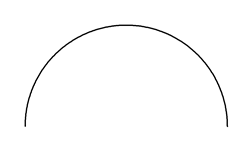
\includegraphics[width=\textwidth]{image/arcpiece1}
			\caption{$n=1$}
		\end{subfigure}
		\begin{subfigure}{.4\textwidth}
			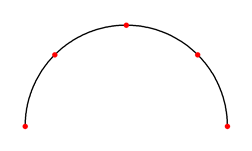
\includegraphics[width=\textwidth]{image/arcpiece2}
			\caption{$n=2$}
		\end{subfigure}
	\end{center} \setstretch{1.2}
    \caption{곡선을 조각별로 나누기}
	\raggedright \small  $n=2$일 때, $\gamma(t)=(\cos\pi{t},\sin\pi{t},0)$으로 매개되는 단위 반윈을 $2^{n}$개의 조각으로 나누기 전(왼쪽)과 후(오른쪽)
\end{figure}


이제 각 조각을 근사할 것이다.
 $\textbf{C}_{i}$위의 한 점에서 $\gamma_{i}(0)$과 $\gamma_{i}(1)$에 내린 수선의 길이가 최대가 되는 점을 중간점이라 정의하고, $\gamma_{i}(t_{1/2})$라 하자. 세 점 $\textbf{P}_{i,0},\textbf{P}_{i,1},\textbf{P}_{i,2}$ 를 다음과 같이 정의한다. 
\begin{equation}
	\begin{split}
	&\textbf{P}_{i,0}=\gamma_{i}(0), \\
	&\textbf{P}_{i,1}=2\gamma_{i}(t_{1/2})-\frac{\gamma_{i}(0)+\gamma_{i}(1)}{2}, \\
	&\textbf{P}_{i,2}=\gamma_{i}(1)
	\end{split}
\end{equation}
이제 $\textbf{P}_{i,0},\textbf{P}_{i,1},\textbf{P}_{i,2}$를 세 조절점으로 가지는 베지어 곡선은 다음과 같이 주어진다.
\begin{equation}
	\begin{split}
		&\beta_{i}(t)=(1-t)^{2}\textbf{P}_{i,0}+2t(1-t)\textbf{P}_{i,1}+t^{2}\textbf{P}_{i,2} \\
		&B_{i}=\beta_{i}([0,1])
	\end{split}
\end{equation}
\begin{figure}[h]
	\centering
	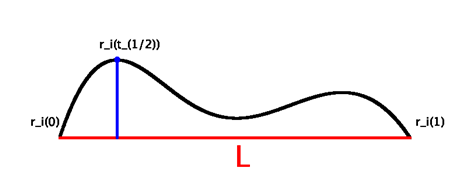
\includegraphics[width=.9\textwidth]{image/BCmiddlepoint}
	\caption{중간점}
	\raggedright
	\small 조각 $\textbf{C}_{i}=\gamma_{i}([0,1])$에서의 중간점은 $\gamma_{i}(0)$과 $\gamma_{i}(1)$을 잇는 직선에 내린 수선의 길이가 최대가 되게 하는  $\textbf{C}_{i}$위의 점을 말하며, $\gamma_{i}(t_{1/2})$로 나타낸다. 
\end{figure}
\begin{figure}[h] \label{8}
	\begin{center}
		\begin{subfigure}{.2\textwidth}
			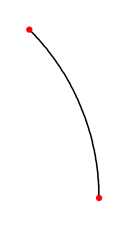
\includegraphics[width=\textwidth]{image/BCstep1}
			\caption{$n=1$}
		\end{subfigure}
		\begin{subfigure}{.2\textwidth}
			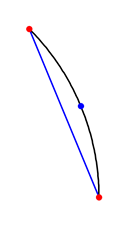
\includegraphics[width=\textwidth]{image/BCstep2}
			\caption{$n=2$}
		\end{subfigure}
		\begin{subfigure}{.2\textwidth}
	    	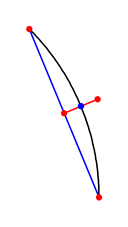
\includegraphics[width=\textwidth]{image/BCstep3}
	        \caption{$n=3$}
    	\end{subfigure}
	    \begin{subfigure}{.2\textwidth}
		    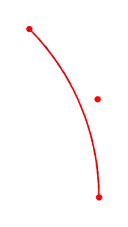
\includegraphics[width=\textwidth]{image/BCstep4}
		    \caption{$n=4$}
	    \end{subfigure}
	\end{center} \setstretch{1.2}
    \caption{각 조각을 근사하기}
	\raggedright \small  조각 $\gamma_{i}([0,1])$, $\gamma_{i}(0)=\textbf(P)_{i,0}$과 $\gamma_{i}(1)=\textbf(P)_{i,2}$을 잇는 직선과 중간점 $\gamma_{i}(t_{1/2})$, 중간점을 이용해 얻은 베지어 곡선의 조절점 $\textbf{P}_{i,1}=2\gamma_{i}(t_{1/2})-\frac{\gamma_{i}(0)+\gamma_{i}(1)}{2}$, 베지어 곡선의 세 조절점 $\textbf{P}_{i,0},\textbf{P}_{i,1},\textbf{P}_{i,2}$를 이용해 그린 2차 베지어 곡선.
\end{figure}
\begin{figure}[h] 
	\centering
	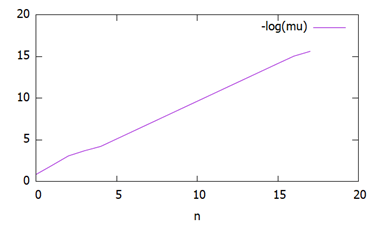
\includegraphics[width=.4\textwidth]{image/BCerror}
	\caption{근사수치} 
	\label{fig:sp}
	\raggedright
	\small 조각 근사 거리: 단위 반원을 근사할 때, $n$의 값에 대한 $-\log\mu$의 그래프. 이 증가함에 따라 $\mu$는 기하급수적으로 감소하는 경향을 보인다. 
\end{figure}
\cref{fig:sp}를 보면 단위 반원을 근사해본 결과 다음 그림과 같은 수치를 알 수 있었고 이를 그래프로 나타낼 수 있었다.
단위 반원의 경우 $n=2$이면 $\log\mu$는 -3.08랑 비슷한 결과가 나타났다.
\subsubsection{수렴성 증명}
\begin{theorem} \label{BCproof2}
	서로 다른 세 점 $\textbf{P}_{0},\textbf{P}_{1},\textbf{P}_{2}$를 조절점으로 가지는 베지어 곡선에 대해 $\textbf{Q}$를 $\eqref{BCmiddle}$와 같이 정의하자. 베지어 곡선 위의 두 점을 잇는 벡터의 $\textbf{P}_{0}$와 $\textbf{P}_{2}$를 잇는 직선에 평행한 성분의 최댓값은 $2\max(\parallel\textbf{P}_{0}-\textbf{Q}\parallel,\parallel\textbf{P}_{2}-\textbf{Q}\parallel)$보다 작거나 같다. 
\end{theorem}
\begin{proof}
	위의 증명과 마찬가지로 2차 베지어 곡선을 포함하는 평면에서 $u,v$축을 설정하자. 일반성을 잃지 않고 $a,b,c>0$이라 할 수 있다. 다음 두 가지 경우가 가능하다.
	\begin{figure}[h]
		\begin{center}
			\begin{subfigure}{.4\textwidth}
				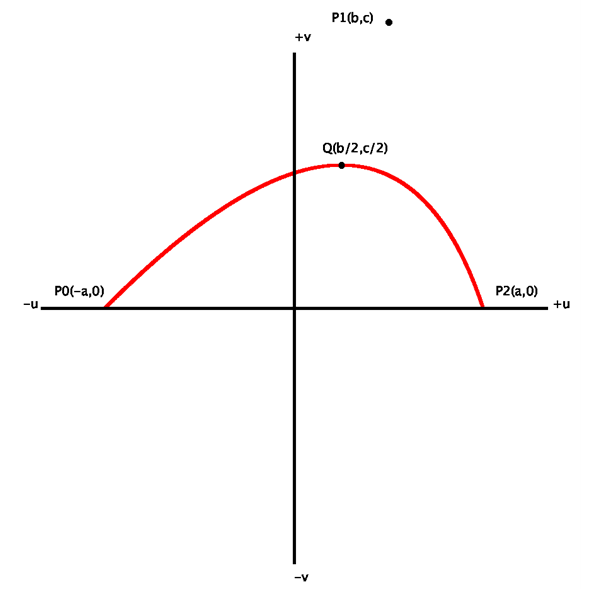
\includegraphics[width=\textwidth]{image/BCcase1}
				\caption{$n=1$}
			\end{subfigure}
			\begin{subfigure}{.4\textwidth}
				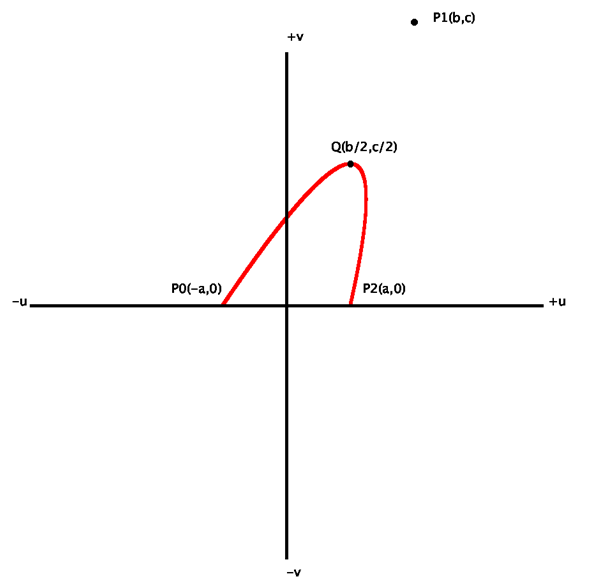
\includegraphics[width=\textwidth]{image/BCcase2}
				\caption{$n=2$}
			\end{subfigure}
		\end{center} \setstretch{1.2}
        \caption{베지어 곡선의 매개화}
		\raggedright \small  베지어 곡선 위의 모든 점은 한 평면상에 존재하기 때문에 축과 축을 설정할 수 있다. 특히, 으로 놓을 수 있다. 일반성을 잃지 않고 이라 할 경우 위 두 가지 경우가 가능하다.
	\end{figure}
	첫 번째 경우 자명하게 최댓값은 $2a$이다.
	\begin{equation}
		2a\leq2\sqrt{{\left(a+\frac{b}{2}\right)^{2}}+{\left(\frac{c}{2}\right)^{2}}}=\parallel\textbf{P}_{0}-\textbf{Q}\parallel
	\end{equation}
	두 번째 경우 베지어 곡선 위의 한 점은 다음과 같이 나타낼 수 있다. 
	\begin{equation}
		\begin{split}
		\textbf{B}(t)&=(1-t)^{2}\textbf{P}_{0}+2t(1-t)\textbf{P}_{1}+t^{2}\textbf{P}_{2} \\
		&=(-a(1-t)^{2}+2bt(1-t)+at^{2},2ct(1-t))
		\end{split}
	\end{equation}
	베지어 곡선 위의 두 점을 잇는 벡터의 $u$성분은 다음 식의 값보다 작거나 같다.
	\begin{equation}
		\begin{split}
		&(-a(1-t)^{2}+2bt(1-t)+at^{2})-(-a) \\
		&=-2bt^{2}+2(a+b)t  \\
		&=-2b\left(t-\frac{a+b}{2b}\right)^{2}+\frac{(a+b)^{2}}{2b}  
		\end{split}
	\end{equation}
	베지어 곡선의 개형이 위와 같으므로 이 이차함수는 $t\in[0,1]$에서 최댓값을 가진다. 따라서$(a+b)/2b\leq{1}$ 이 성립하고 이는 $a\leq{b}$와 같다.
	\begin{equation}
		\begin{split}
			&\frac{(a+b)^{2}}{2b}=\frac{a^{2}}{2b}+a+\frac{b}{2}\leq\frac{b}{2}+a+\frac{b}{2}=a+b \\
			&2\parallel\textbf{P}_{0}-\textbf{Q}\parallel=2\sqrt{\left(a+\frac{b}{2}\right)^{2}+\left(\frac{c}{2}\right)^{2}}\geq2a+b
		\end{split}
	\end{equation}
	따라서
	\begin{equation}
		\frac{(a+b)^{2}}{2b}\leq{a+b}\leq{2a+b}\leq{2\parallel\textbf{P}_{0}-\textbf{Q}\parallel}
	\end{equation}
\end{proof}
이제 지금까지 소개했던 성질들을 이용하여 충분한 근사가능성에 관한 것을 증명할 것이다.
임의의 $\epsilon>0$에 대해 $\mu<\epsilon$이 성립하는 $n$이 존재한다는 것은 $\lim_{n\to\infty} \mu =0$의 필요조건이다. 즉, 충분한 근사 가능성에 대한 연구의 방향은  $\lim_{n\to\infty} \mu =0$을 증명하는 것을 목표로 한다. $\mu$의 정의에 따라 모든 $i=0,1,\cdots,2^{n}-1$에 대해 $\lim_{n\to\infty} \mu_{i} =0$을 보이는 것과 같다.

 $\mu_{i}=d_{H}(C_{i},B_{i})$는 계산하기 어렵지만 $d_{H}(C_{i},L)$과 $d_{H}(B_{i},L)$은 할 수 있다. 여기서 $L$은 조각의 양 끝점을 잇는 선분이다. 직관적으로 $n$이 충분히 크면 $C$와 $B$가 연속함수의 상이므로 $d_{H}(C_{i},L)$와 $d_{H}(B_{i},L)$ 이 모두 $0$으로 수렴할 것으로 예상된다. 그래서 연속함수의 정의인 $\epsilon-\delta$ 논법을 이용하여 이를 증명한다.
 
 
이 근사거리를 통한 오차 분석의 신뢰성은 높다. 여기서 근사 거리는 원래 곡선과 근사한 곡선 사이의 하우스도르프 거리로 정의한다. 하우스도르프 거리는 거리공간 $(\textbf{M},d)$의 두 부분집합이 얼마나 멀리 있는가를 나타낸다. $d_{H}(\textbf{X},\textbf{Y})=0$일 필요충분조건은 $\textbf{X}$와 $\textbf{Y}$가 동일한 폐포를 가지는 것으로, $\textbf{X},\textbf{Y}$가 닫힌 집합일 때는 $\textbf{X}=\textbf{Y}$와 동치이다. 따라서 하우스도르프 거리는 본 연구에서 두 곡선 사이의 오차를 나타내기 충분하다. 베지어 곡선으로 원호를 근사하는 선행 연구에서도 하우스도르프 거리를 사용했으므로 그 신뢰성도 높다. \cite{Seon-Hong Kim}
\begin{theorem}\label{2Dproof}
	임의의 곡선 $C$와 위 방법에 따라 얻은 $B$ 사이의 근사거리 $\mu$에 대해 다음이 성립한다.
	\begin{equation}
		\lim_{n\to\infty}\mu=0
	\end{equation}
\end{theorem}
\begin{lemma}
	거리공간 $(M,d)$의 공집합이 아닌 유계인 세 닫힌 부분집합 $X,Y,Z$에 대해 다음이 성립한다.
	\begin{equation}
		d_{H}(X,Y)\leq{d_{H}(X,Z)+d_{H}(Z,Y)}
	\end{equation}
\end{lemma}
\begin{proof}
	먼저 $d(x,Y)=inf_{y\in{Y}}d(x,y)$와 $d(X,Y)=sup_{x\in{X}}d(x,Y)$에 대해
	\begin{equation}
		d(x.Y)\leq{d(x,Z)+d(Y,Z)}
	\end{equation}
    가 성립함을 보이자
    \begin{equation}
    	\begin{split}
    		&d(x,Z)=\inf_{z\in{Z}}d(x,z)=\min_{z\in{Z}}d(x,z)=d(x,z_{0}) \ (z_{0}\in{Z})  \\
    		&d(z_{0},Y)=\inf_{y\in{Y}}d(z_{0},y)=\min_{y\in{Y}}d(z_{0},y)=d(z_{0},y_{0}) \ (y_{0}\in{Y})
    	\end{split}
    \end{equation}
따라서
    \begin{equation}
	    \begin{split}
		   d(x,Y)&\leq{d(x,y_{0})}  \\
		   &\leq{d(x,z_{0})+d(z_{0},y_{0})}  \\
		   &=d(x,Z)+d(z_{0},Y)  \\
		   &\leq{d(x,Z)+d(Z,Y)}
     	\end{split}
    \end{equation}
$x\in{X}$에 대해서 
   \begin{equation}
     	\begin{split}
		d(x,Y)&\leq{d(x,Z)+d(Z,Y)}  \\
		&\leq{d(X,Z)+d(Z,Y)}  \\
		&\leq{max(d(X,Z),d(Z,X))+max(d(Z,Y),d(Y,Z))}  \\
		&=d_{H}(X,Z)+d_{H}(Z,Y)
     	\end{split}
   \end{equation}
   \begin{equation}
   	d(X,Y)\leq{\sup_{x\in{X}}d(x,Y)}\leq{d_{H}(X,Z)+d_{H}(Z,Y)}
   \end{equation}
비슷하게 $d(Y,X)\leq{d_{H}(X,Z)+d_{H}(Z,Y)}$를 얻을 수 있다.
   \begin{equation}
   	d_{H}(X,Y)=max(d(X,Y),d(Y,X))\leq{d_{H}(X,Z)+d_{H}(Z,Y)}
   \end{equation}
\end{proof}
이제 \cref{2Dproof}에 대한 증명은 다음과 같다.
\begin{proof}
	각 $i=0,1,\cdots,2^{n}-1$에 대해서
	
	L을 $\gamma_{i}(0)$와 $\gamma_{i}(1)$을 잇는 선분이라 가정하자.
	
	$\gamma_{i}(t_{1/2})$에서 $L$을 포함한 직선에 내린 수선의 길이를 $h$라 하면 
	\begin{equation*}
		d_{H}(C_{i},L)\leq{\sup_{c\in{C_{i}}}\sup_{l\in{L}}\parallel\textbf{c}-\textbf{l}\parallel}
	\end{equation*}
$\parallel\textbf{c}-\textbf{l}\parallel$에서 $L$에 수직인 성분의 최댓값은 정의에 따라 $h$이다. $L$에 평행한 성분의 최댓값은 $\max(\max_{t\in[0,1]}\parallel\gamma_{i}(t)-\gamma_{i}(0)\parallel,\max_{t\in[0,1]}\parallel\gamma_{i}(t)-\gamma_{i}(1)\parallel)$보다 작거나 같다.
\begin{figure}[h]
	\begin{center}
	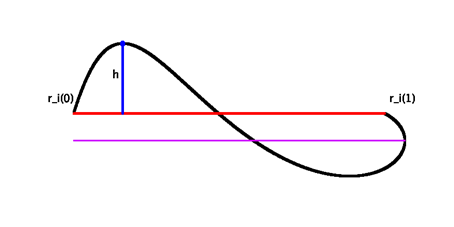
\includegraphics[width=.7\textwidth]{image/BCproof1}
	\caption{L에 평행한 성분}
    \end{center} \setstretch{1.2}
	\small\raggedright 
	$\gamma_{i}(0)$과 $\gamma_{i}(1)$을 잇는 선분 $L$(빨간색). $\textbf{c}\in{C_{i}},\textbf{l}\in{L}$에 대해 $\parallel\textbf{c}-\textbf{l}\parallel$의 $L$에 수직인 성분의 최댓값은 $h$(파란색), $L$에 평행한 성분의 최댓값은 보라색 선분의 길이와 같다.
\end{figure}
\begin{equation}
  \begin{split}
   d_{H}(C_{i},L)&\leq\sup_{\textbf{c}\in{C_{i}}}\sup_{\textbf{l}\in{L}}\parallel\textbf{c}-\textbf{l}\parallel \\
   &\leq{h+\max\left(\max_{t\in[0,1]}\parallel\gamma_{i}(t)-\gamma_{i}(0)\parallel,\max_{t\in[0,1]}\parallel\gamma_{i}(t)-\gamma_{i}(1)\parallel\right)} \\
   &\leq{2\max\left(\max_{t\in[0,1]}\parallel\gamma_{i}(t)-\gamma_{i}(0)\parallel,\max_{t\in[0,1]}\parallel\gamma_{i}(t)-\gamma_{i}(1)\parallel\right)}
  \end{split}
\end{equation}
중간 조절점을 설정한 과정 \cref{BCproof2}에서 우리는 $B_{i}$위의 한 점에서 $L$을 포함한 직선에 내린 수선의 길이의 최댓값도 $h$인것을 알 수 있다.
\begin{equation}
	\begin{split}
		d_{H}(B_{i},L)&\leq\sup_{\textbf{b}\in{B_{i}}}\sup_{\textbf{l}\in{L}}\parallel\textbf{b}-\textbf{l}\parallel \\
		&\leq{h+2\max\left(\parallel\gamma_{i}(t_{1/2})-\gamma_{i}(0)\parallel,\parallel\gamma_{i}(t_{1/2})-\gamma_{i}(1)\parallel\right)} \\
		&\leq{3\max\left(\parallel\gamma_{i}(t_{1/2})-\gamma_{i}(0)\parallel,\parallel\gamma_{i}(t_{1/2})-\gamma_{i}(1)\parallel\right)} \\
		&\leq{3\max\left(\max_{t\in{[0,1]}}\parallel\gamma_{i}(t)-\gamma_{i}(0)\parallel,\max_{t\in{[0,1]}}\parallel\gamma_{i}(t)-\gamma_{i}(1)\parallel\right)}
	\end{split}
\end{equation}
따라서
\begin{equation}
	\begin{split}
		d_{H}(C_{i},B_{i})&\leq{d_{H}(C_{i},L)+d_{H}(C_{i},L)} \\
		&\leq{5\max\left(\max_{t\in{[0,1]}}\parallel\gamma_{i}(t)-\gamma_{i}(0)\parallel,\max_{t\in{[0,1]}}\parallel\gamma_{i}(t)-\gamma_{i}(1)\parallel\right)}
	\end{split}
\end{equation}
$\gamma(t)$가 연속이므로 임의의 $\epsilon>0$에 대해 다음을 만족하는 $\delta_{i,0},\delta_{i,1}>0$이 존재한다.
\begin{equation}
	\begin{split}
	\left|t-\frac{i}{2^{n}}\right|<\delta_{i,0}&\Longrightarrow\left\Vert\gamma(t)-\gamma\left(\frac{i}{2^{n}}\right)\right\Vert<\frac{\epsilon}{5} \\
	\left|t-\frac{i+1}{2^{n}}\right|<\delta_{i,1}&\Longrightarrow\left\Vert\gamma(t)-\gamma(\frac{i+1}{2^{n}})\right\Vert<\frac{\epsilon}{5}
	\end{split}
\end{equation}
이제 $N_{i}$를 $2^{N_{i}}>\max(1/\delta_{i,0},1/\delta_{i,1})$를 만족하는 최소의 양의 정수로 정의하자

$n>N_{i}$에 대해

$1/2^{n}<\delta_{i,0}$이므로 $t\in{[0,1]}$에 대해 $\mid\frac{i+t}{2^{n}}-\frac{i}{2^{n}}\mid<\delta_{i,0}$
\begin{equation}
     \parallel\gamma_{i}(t)-\gamma_{i}(0)\parallel=\left\Vert\gamma\left(\frac{i+t}{2^{n}}\right)-\gamma\left(\frac{i}{2^{n}}\right)\right\Vert<\frac{\epsilon}{5}
\end{equation}
마찬가지로 $\parallel\gamma_{i}(t)-\gamma_{i}(1)\parallel<\frac{\epsilon}{5}$를 얻을 수 있다.

따라서 $n>N_{i}$이면 $\mu_{i}=d_{H}(C_{i},B_{i})<\epsilon$이다. 

$N=\max^{2^{n}-1}_{i=0}N_{i}$라 정의하면 $n>N \Longrightarrow{}\max^{2^{n}-1}_{i=0}\mu_{i}<\epsilon$
\begin{equation}
	\therefore\lim_{n \to \infty}\mu=0
\end{equation}
\end{proof}
이 증명을 통해 우리는 근사 거리는 항상 분할하는 횟수가 늘어감에 따라 0으로 수렴함을 알 수 있었다. 그러므로 우리는 임의의 연속된 곡선에 대해 충분한 근사가 항상 가능하다고 결론 지을 수 있다.
\subsection{3D model improvement} \label{last research}
이제 2D 모델 근사에 대한 방법을 알아보았으니 3D 모델도 비슷하게 근사가 가능하다는 것을 보여줄 것이다. 
\subsubsection{분할 방법}
주어진 모델을 하나의 베지어 곡면으로 나타내려면 오차가 너무 커진다. 그래서 우리는 obj 파일의 정점 혹은 point cloud를 분할하고, 분할된 각 영역의 곡면을 하나의 베지어 곡면으로 근사하는 방법을 택했다. 이를 위해 고안한 두 가지 분할 방법이 있다. 
\begin{itemize}
	\item \textbf{8진 트리.} 8진 트리는 카테시안 좌표계를 기준으로 하며, 원점(기준점)에 대해 공간을 $xy$평면, $yz$평면, $zx$평면으로 잘라 8개의 영역으로 나누는 방식이다. 8개 영역으로 분할되기 때문에 8개의 자식 노드가 생긴다고 볼 수 있다. 8진 트리 방식의 장점은 모델의 제한 없이 항상 적용 가능하다는 점이다. 그러나 분할된 조각을 베지어 곡면으로 근사하기 어렵고, 조각이 8배씩 많아지므로 시간이 오래 걸린다.
	
	\item \textbf{원통형 분할.} 원통형 분할은 원통형 좌표계를 기준으로 하며, $(r, \theta, z)$로 표현되는 정점들을 $\theta$와 $z$에 따라 나눈다. $\theta-z$ 평면에 각 정점들을 표현하고 $4^n$등분하여 영역을 분할하는 방식이다. 원통형 분할은 같은 $(\theta, z)$ 값에 대해 두 개 이상의 점이 존재하면 적용할 수 없다는 단점이 있다. 그러나 8진 트리 방법보다 시간이 적게 소모되고, 최종적으로 만들어진 곡면을 조각적으로 정의된 연속함수 $\mathbf{x}^*\colon\mathbb{R}^2\to\mathbb{R}^3$에 대해 $\mathbf{x}^*([0, 1]^2)$으로 표현할 수 있다는 장점이 있다. 이 점은 모델의 RGB 색을 압축할 때도 사용될 수 있다. 
\end{itemize}
우리는 원통형 분할을 이용하기로 결정했다. 또한 위에서 설명한 단점을 없애기 위해 연구 대상을 축소했다. $\mathbb{R}^3$의 볼록 집합의 경계로 표현되는 곡면만을 근사한다. \cref{homeo}에 따라 이는 2차원 곡면이 된다. 

원통형 분할을 하기 앞서 몇 가지 사전 작업이 필요하다. 정점 $\mathbf{P}_k$ 중 가장 거리가 먼 두 정점을 $z$축 위에 올리는 일이다. 원점이 모델 밖에 있으면 같은 $(\theta, z)$에 대해 두 개 이상의 점이 존재할 수 있다. 또는 기울어진 타원체를 생각하면, 거리가 가장 먼 두 점이 $z$축 위에 있는 게 좋다는 걸 알 수 있다. 또한 원기둥의 밑면과 같이 $z$축에 수직인 면이 문제가 될 수 있지만, 이 작업을 통해 이런 문제를 해결할 수 있다. 

가장 거리가 먼 두 점을 $(x_1, y_1, z_1), (x_2, y_2, z_2)$라 하자. 각 정점을 평행이동하여 두 점의 중심이 원점에 오게 한다. 아래의 과정은 모두 우변의 항을 좌변에 대입한다고 할 때 성립하는 식이다.
\begin{equation*}
	\mathbf{P}_k = 
	 \mathbf{P}_k - \left(\frac{x_1+x_2}2,\ \frac{y_1+y_2}2,\ \frac{z_1+z_2}2\right)^\intercal
\end{equation*}
이제 $xy$ 회전, $yz$ 회전을 통해 두 점을 $z$축 위로 올린다. 각각 다음과 같다. 
\begin{align*}
	\mathbf{P}_k\ =\ \begin{pmatrix}
		x_1 & y_1 & 0 \\ -y_1 & x_1 & 0 \\ 0 & 0 & 1
	\end{pmatrix} \mathbf{P}_k \\
	\mathbf{P}_k\ =\ \begin{pmatrix}
		z_1 & 0 & -x_1 \\ 0 & 1 & 0 \\ x_1 & 0 & z_1
	\end{pmatrix} \mathbf{P}_k
\end{align*}
최종적으로 거리가 가장 먼 두 점의 좌표를 $(0, 0, \pm h)$라 한다. \\

$\theta$와 $z$의 범위는 각각 $0\leq \theta <2\pi$, $-h \leq z \leq h$이므로, 원통형 분할을 하면 각 영역은 $\theta_i=2\pi i/2^n,\ z_j=-h+2hj/2^n\ (0\leq i, j < 2^n)$을 경계로 한다. 

\subsubsection{Control Point Determination}\label{2.2}
분할된 곡면을 근사하는 베지어 곡면을 결정하기 위해서 9개의 조절점이 필요하다. 결정된 베지어 곡면이 연속적으로 이어지기 위해서는 $\mathbf{b}_{11}$를 제외한 나머지 조절점은 영역 안에 있는 정점들과는 무관하게 결정되어야 한다. 각 영역의 경계는 $\theta=\theta_i$ 혹은 $z=z_j$로 주어지므로, 직선 $\ell \colon \theta=\theta_i, z=z_j$와 obj 파일의 면 $F$의 교점으로 네 조절점 $\mathbf{b}_{00}, \mathbf{b}_{02}, \mathbf{b}_{20}, \mathbf{b}_{22}$를 구한다. 여기서 직선과 삼각형의 교점을 찾는 빠른 알고리즘인 Möller-Trumbore intersection algorithm을 사용한다.\cite{raytriangle} 우리는 2D model 근사에서 중간 조절점을 잡은 방법을 이용하여 네 조절점 $\mathbf{b}_{01}, \mathbf{b}_{10}, \mathbf{b}_{12}, \mathbf{b}_{21}$을 얻을 수 있다. (2,2)차 베지어 곡면에서, $u=0,\ u=1,\ v=0,\ v=1$인 부분은 각각 2차 베지어 곡선이 되기 때문이다. 두 영역의 경계 $\theta=\theta_i, z\in[z_j, z_{j+1}]$ 혹은 $F$들의 교선을 하나의 2차 베지어 곡면으로 근사하면 된다. \cref{3D control}은 $\mathbf{b}_{11}$을 제외한 8개의 점을 고른 사진이다.

\begin{figure}[h]
	\centering
	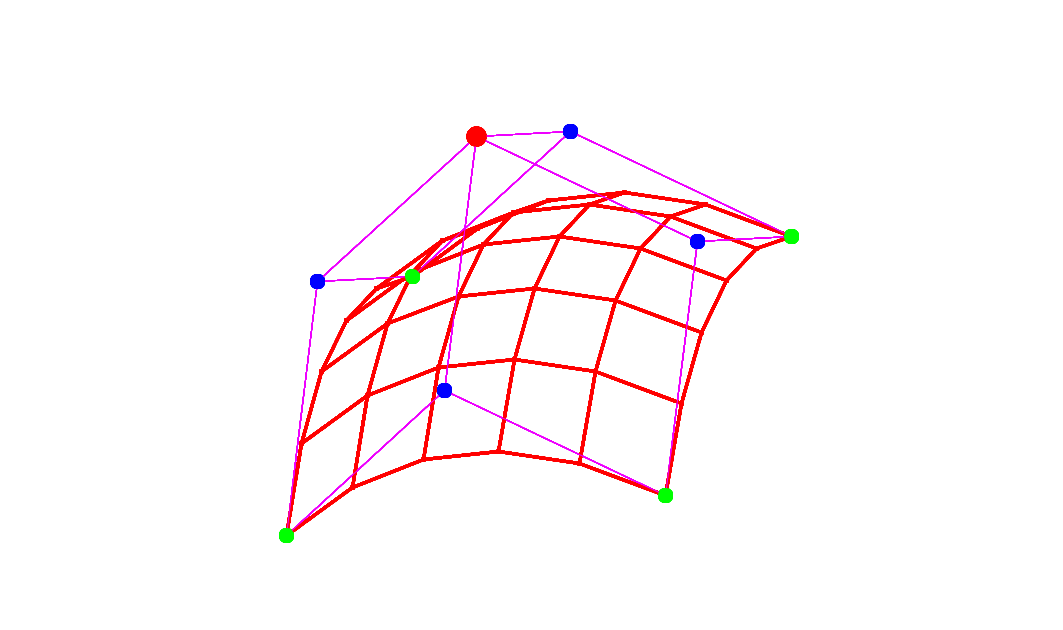
\includegraphics[width=.8\textwidth]{image/22BS}
	\caption{$(2,2)$-차 베지어 곡면}
	\small $(2,2)$-차 베지어 곡면은 네 모서리가 결정되면 하나의 조절점만 정할 수 있다. 
	\label{3D control}
\end{figure}
$\mathbf{b}_{11}$을 구하기 위해 최소제곱법을 이용한다. 
최소제곱법을 이용하는 아이디어는 선행 연구를 참조했다.\cite{2021} 최소제곱법을 사용하기 위해서는 obj 파일의 각 정점 $\mathbf{P}_k$에 대응되는 베지어 곡면 위의 점 $\mathbf{x}_k=\mathbf{x}(u_k, v_k)$을 알아야 한다. 이미 알고 있는 8개 조절점에 대한 항을 $\mathbf{y}_k$라 하면 다음과 같이 나타낼 수 있다. 
\begin{equation*}
	\mathbf{x}_k=B_1^2(u_k)B_1^2(v_k)\mathbf{b}_{11}+\mathbf{y}_k
\end{equation*}
이제 $\mathbf{x}_k=\mathbf{P}_k\ (k=1, \cdots, K)$의 제곱오차 $S=\sum_{k=1}^K \| \mathbf{x}_k-\mathbf{P}_k \|^2$를 최소화하기 위해 행렬방정식으로 나타낸다.
\begin{equation*}
	\begin{pmatrix}
		B_1^2(u_1)B_1^2(v_1) \\ B_1^2(u_2)B_1^2(v_2) \\ \vdots \\ B_1^2(u_K)B_1^2(v_K)
	\end{pmatrix} \begin{pmatrix}
		b_{11}^x & b_{11}^y & b_{11}^z
	\end{pmatrix} = \begin{pmatrix}
		P_1^x-y_1^x & P_1^y-y_1^y & P_1^z-y_1^z \\ P_2^x-y_2^x & P_2^y-y_2^y & P_2^z-y_2^z \\ \vdots & \vdots & \vdots \\ P_K^x-y_K^x & P_K^y-y_K^y & P_K^z-y_K^z
	\end{pmatrix}
\end{equation*}
이때 윗첨자 $x, y, z$는 각각 벡터의 $x, y, z$성분을 가르킨다. 이 경우에도 제곱오차는 마찬가지로 $S$이다. $AX=B$ 꼴의 행렬방정식에서 최소제곱오차를 가지는 $\hat{X}$는 $\hat{X}=(A^\intercal A)^{-1}A^\intercal B$로 주어지므로, $\mathbf{b}_{11}$을 다음과 같이 근사할 수 있다. 
\begin{equation} \label{firstfindb11}
	\mathbf{b}_{11}=\dfrac{\sum_{k=1}^K B_1^2(u_k)B_1^2(v_k)(\mathbf{P}_k-\mathbf{y}_k)}{\sum_{k=1}^K (B_1^2(u_k)B_1^2(v_k))^2}
\end{equation}
각 $k$에 대해 $u_k$와 $v_k$의 값을 안다면 \eqref{firstfindb11}과 같이 $\mathbf{b}_{11}$을 구할 수 있다. 이제 최적의 $u_k, v_k$를 찾기 위해 뉴턴-랩슨 방법을 이용한다. 뉴턴-랩슨 방법을 적용할 함수는 $\mathbf{x}-\mathbf{P}_k$이다. 즉 현재 $u_{n, k}$와 $v_{n, k}$가 주어질 때, 다음과 같이 $u_{n+1, k}$와 $v_{n+1, k}$를 얻는다. 
\begin{align} \label{rearrangeu}
	u_{n+1, k}&=u_{n, k}-\frac{\mathbf{x}-\mathbf{P}_k}{\partial(\mathbf{x}-\mathbf{P}_k)/\partial u} \bigg|_{u=u_{n, k}} \\
	v_{n+1, k}&=v_{n, k}-\frac{\mathbf{x}-\mathbf{P}_k}{\partial(\mathbf{x}-\mathbf{P}_k)/\partial v} \bigg|_{v=v_{n, k}} \label{rearrangev}
\end{align}
그런데 벡터의 나눗셈은 정의되지 않으므로 이번에도 최소제곱법을 이용한다. 즉 $[\partial(\mathbf{x}-\mathbf{P}_k)/\partial u] \Delta u = \mathbf{x}-\mathbf{P}_k$의 제곱 오차를 최소로 하는 스칼라 $\Delta u$를 선택한다. 
초기 조건 $u_{0, k}=v_{0, k}=0.5$에 대해 $\mathbf{b}_{11}$를 구하고 새로 $u_k, v_k$를 구하는 과정을 반복한다. 
다음 사진의 과정을 통해 위 과정을 20번 반복하면 $u_k$와 $v_k$의 값이 거의 일정 한 것을 알아냈다.


\begin{figure}[h]
	\centering
	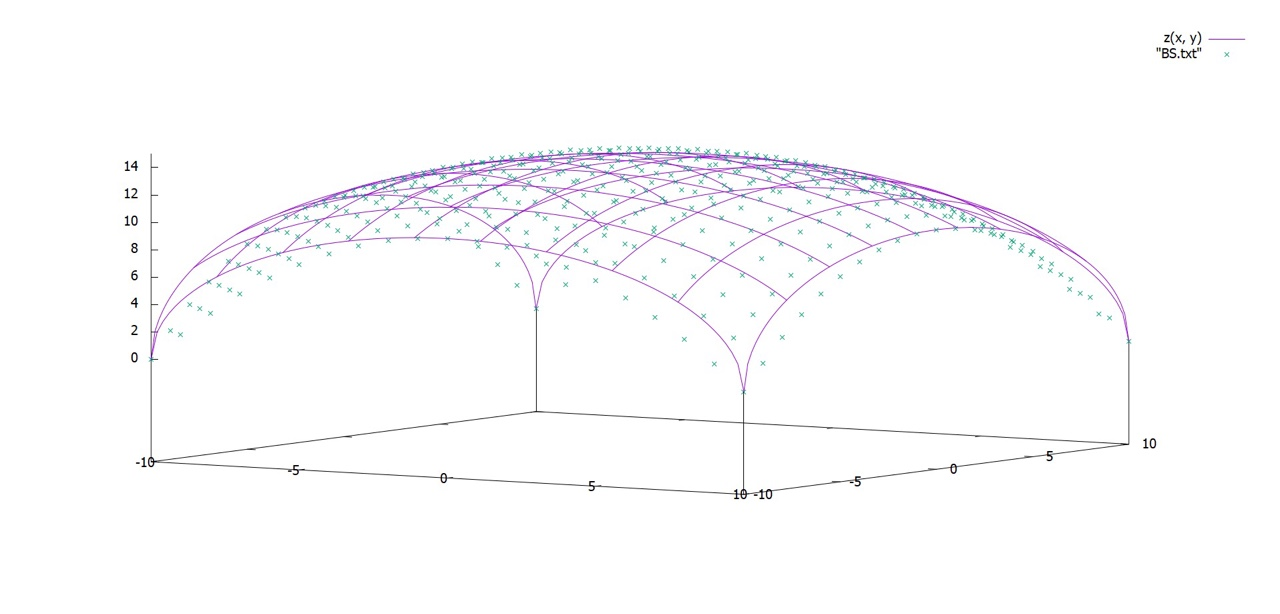
\includegraphics[width=\textwidth]{image/leastSquare}
	\caption{근사 방법}
	\label{gnuplot}
	\raggedright\small 곡면 $z=\sqrt{200-x^2-y^2}\ (-10 \leq x, y \leq 10)$에 위 근사 방법을 적용한 예시이다. 곡면 위 점의 개수는 $K=100$이며 $\mathbf{P}_k$는 $x$와 $y$의 좌표가 $((2i-9)/10,\ (2j-9)/10)\ (i, j = 0, 1, \cdots, 9)$인 점이다. 이때 곡면과 근사한 베지어 곡면 사이의 하우스도르프 거리는 약 6.32이다.
\end{figure}
\subsubsection{Algorithm}
  본 연구에서는 어떠한 3D 모델이 있을때 원통형 분할을 이용해 근사를 시작할 것이다. 다음 사진은 원통형 분할을 과정을 시각적으로 보여준 것이다.
  \\
\begin{figure}[h]
	\begin{center}
		\begin{subfigure}{.3\textwidth}
			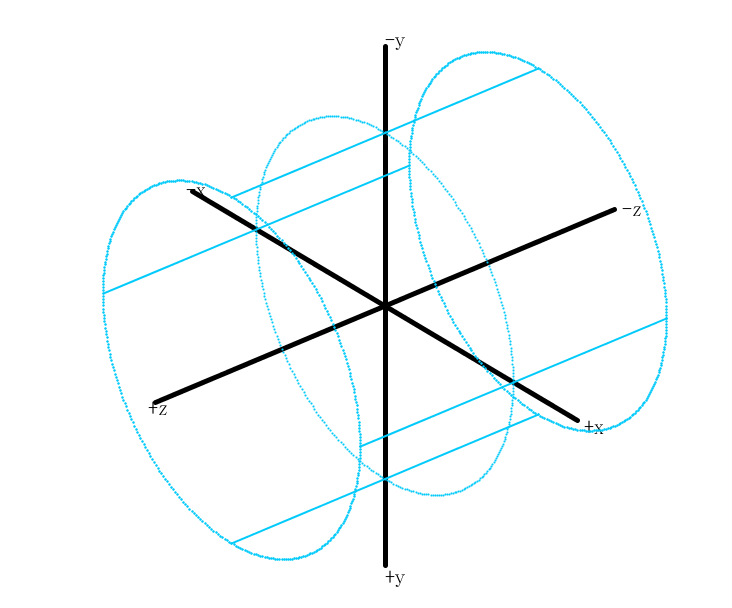
\includegraphics[width=\textwidth]{image/subdivision1}
			\caption{$n=1$}
		\end{subfigure}
		\begin{subfigure}{.3\textwidth}
			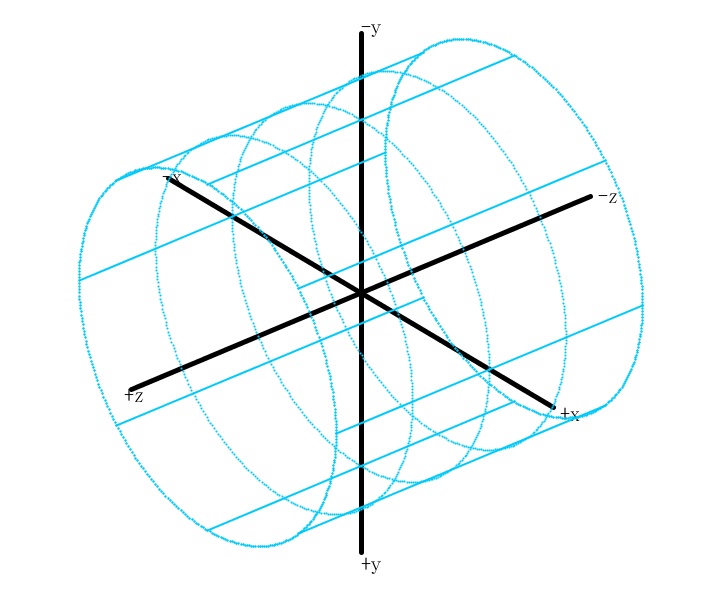
\includegraphics[width=\textwidth]{image/subdivision2}
			\caption{$n=2$}
		\end{subfigure}
		\begin{subfigure}{.3\textwidth}
			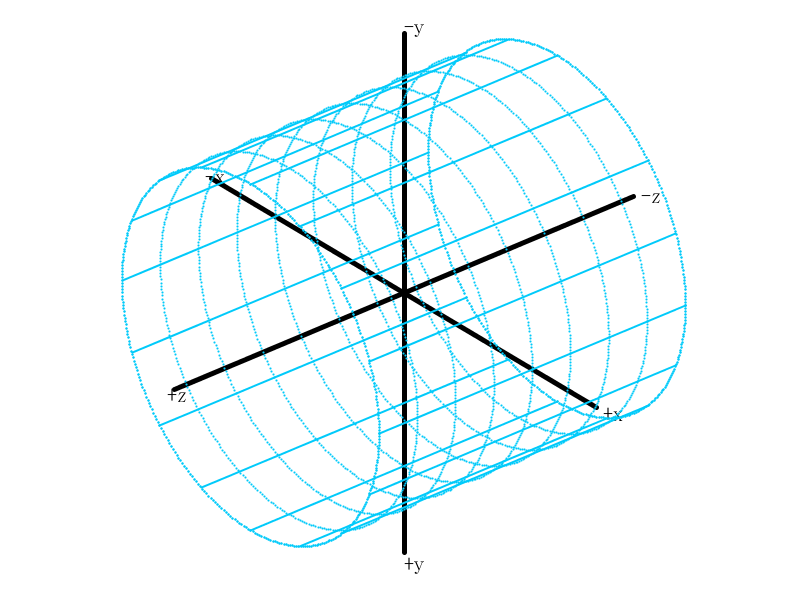
\includegraphics[width=\textwidth]{image/subdivision3}
			\caption{$n=3$}
		\end{subfigure}
	\end{center} \setstretch{1.2}
    \caption{원통형 분할}
	\raggedright \small 원통형 분할은 $\theta$와 $z$의 범위를 이등분하며 이루어진다. 그림에서는 $\theta$와 $z$의 범위를 각각 $2^{n+1}$, $2^n$등분했다. 
\end{figure}

분할된 영역의 곡면을 하나의 베지어 곡면으로 근사한다. 각 영역의 베지어 곡면이 연속적으로 이어지기 위해서는 베지어 곡면의 네 모서리($u=0, \, u=1, \, v=0, \, v=1$)가 영역의 경계에 위치해야 한다. 특히 네 조절점 $\mathbf{b}_{00} = \mathbf{x}(0, 0), \, \mathbf{b}_{02} = \mathbf{x}(0, 1), \, \mathbf{b}_{20} = \mathbf{x}(1, 0), \, \mathbf{b}_{22} = \mathbf{x}(1, 1)$는 각각 4개의 영역이 만나는 경계에 위치한다. 

분할된 영역이 $\theta_a \leq \theta \leq \theta_{a+1}, \, z_b \leq z \leq z_{b+1}$로 주어진다고 하자. 반직선 $\ell_{ab} \colon \theta = \theta_a, \, z = z_b$로 정의하고, 네 반직선 $\ell_{ab}, \, \ell_{a, \, b+1}, \, \ell_{a+1, \, b}, \, \ell_{a+1, \, b+1}$과 obj파일의 면 $F$의 교점을 찾아 각각 $\mathbf{b}_{00}, \mathbf{b}_{02}, \mathbf{b}_{20}, \mathbf{b}_{22}$로 둔다. 이때 광선 또는 직선과 삼각형의 교점을 찾는 빠른 알고리즘인 Möller-Trumbore intersection algorithm을 이용한다. \cite{raytriangle}

Möller-Trumbore intersection algorithm을 이용하면 영역의 경계 $\theta_a \leq \theta \leq \theta_{a+1}, \, z = z_b$와 $F$의 교선을 찾을 수 있다. 식 \eqref{BezierSurface}로 매개화되는 베지어 곡면에서 $u = 0$인 부분은 $\mathbf{b}_{00}, \mathbf{b}_{01}, \mathbf{b}_{02}$를 세 조절점으로 가지는 $2$차 베지어 곡선이다. 다음 2차 베지어 곡선의 성질\eqref{BCmiddle}을 이용하면 $\mathbf{b}_{01}$을 얻을 수 있다. 영역의 경계 $\theta_a \leq \theta \leq \theta_{a+1}, \, z = z_b$와 $\partial C$의 교선을 잡고, 교선 위의 점들 중 $\mathbf{b}_{00}$과 $\mathbf{b}_{02}$를 잇는 직선에서 가장 멀리 떨어진 점 $\mathbf{Q}$를 찾는다. 그러면 $\mathbf{b}_{01} = 2\mathbf{Q} - (\mathbf{b}_{00} + \mathbf{b}_{02})/2$로 주어진다. 같은 방법으로 조절점 $\mathbf{b}_{01}, \mathbf{b}_{10}, \mathbf{b}_{12}, \mathbf{b}_{21}$을 얻을 수 있고 이를 시각적으로 나타내면 다음과 같다. 
\begin{figure}[h]
	\begin{center}
		\begin{subfigure}{.35\textwidth}
			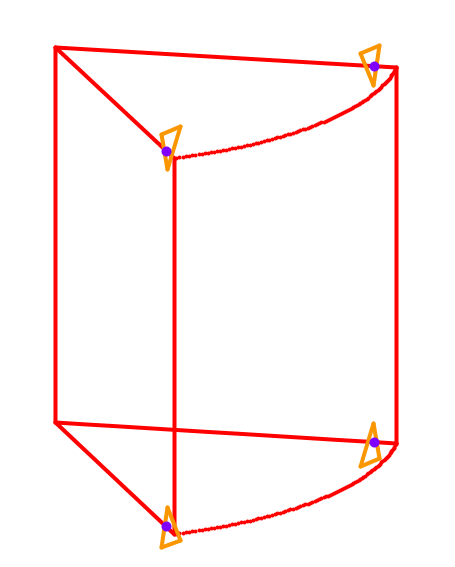
\includegraphics[width=\textwidth]{image/approx1}
			\caption{$\mathbf{b}_{00}, \mathbf{b}_{02}, \mathbf{b}_{20}, \mathbf{b}_{22}$}
		\end{subfigure}
		\begin{subfigure}{.35\textwidth}
			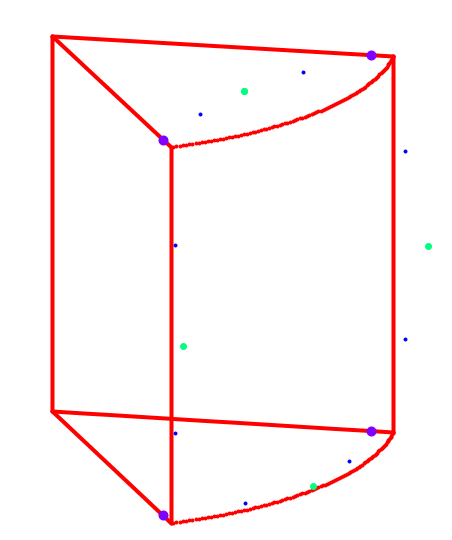
\includegraphics[width=\textwidth]{image/approx2}
			\caption{$\mathbf{b}_{01}, \mathbf{b}_{10}, \mathbf{b}_{12}, \mathbf{b}_{21}$}
		\end{subfigure}
	\end{center} \setstretch{1.2}
	\raggedright \small 
	\caption{조절점}$\mathbf{b}_{11}$을 제외한 조절점을 얻기 위해 Möller-Trumbore intersecton algorithm을 이용한다. (a) 네 영역이 만나는 (반)직선과 obj파일의 면 $F$의 교점으로 $\mathbf{b}_{00}, \mathbf{b}_{02}, \mathbf{b}_{20}, \mathbf{b}_{22}$를 얻는다. (b) 영역의 경계와 $F$의 교선을 잡고, 2차 베지어 곡선을 성질을 이용해 $\mathbf{b}_{01}, \mathbf{b}_{10}, \mathbf{b}_{12}, \mathbf{b}_{21}$를 구한다. 
\end{figure}
이제 조절점 $\mathbf{b}_{11}$을 구하기 위해 최소제곱법과 가우스-뉴턴 방법을 이용한다. 이 과정은 선형 연구를 참고했다. \cite{2021} 영역 내의 정점을 $\mathbf{P}_k \ (k=1, 2, \cdots, K)$라 하자. 각 $\mathbf{P}_k$에 대응되는 베지어 곡면의 매개변수 $u_k$와 $v_k$가 주어졌다고 가정한다. $\mathbf{x}_k = \mathbf{x}(u_k, v_k)$에서 이미 알고 있는 조절점들에 대한 항을 $\mathbf{y}_k$로 두면 다음과 같이 나타날 수 있다.

$$ \mathbf{x}_k = \mathbf{x}(u_k, v_k) = B_1^2(u_k) B_1^2(v_k) \mathbf{b}_{11} + \mathbf{y}_k $$ 

$\mathbf{b}_{11}$에 관한 연립방정식 $\mathbf{x}_k = \mathbf{P}_k \ (1 \leq k \leq K)$는 일반적으로 해를 가지지 않는다. 따라서 제곱오차 $S = \sum_{k=1}^K \Vert \mathbf{x}_k - \mathbf{P}_k \Vert^2$을 최소로 만드는 $\mathbf{b}_{11}$의 값을 구한다. 이를 위해 $x, y, z$ 좌표로 나눠 행렬방정식으로 표현한다. 
\begin{align*}
	&\begin{pmatrix}
		B_1^2(u_1)B_1^2(v_1) \\ B_1^2(u_2)B_1^2(v_2) \\ \vdots \\ B_1^2(u_K)B_1^2(v_K)
	\end{pmatrix} \begin{pmatrix}
		b_{11}^x & b_{11}^y & b_{11}^z
	\end{pmatrix}
	= \begin{pmatrix}
		P_1^x-y_1^x & P_1^y-y_1^y & P_1^z-y_1^z \\ P_2^x-y_2^x & P_2^y-y_2^y & P_2^z-y_2^z \\ \vdots & \vdots & \vdots \\ P_K^x-y_K^x & P_K^y-y_K^y & P_K^z-y_K^z
	\end{pmatrix}
\end{align*}
이때 윗첨자 $x, y, z$는 각각 벡터의 $x, y, z$성분을 나타낸다. 위 행렬방정식의 제곱오차도 마찬가지로 $S$임을 알 수 있다. $AX = B$ 꼴의 행렬방정식에서 최소제곱오차를 가지는 $X = (A^\intercal A)^{-1} A^\intercal B$로 주어지므로, 다음과 같이 $\mathbf{b}_{11}$을 구할 수 있다. 
\begin{equation} \label{secondfindb11}
	\mathbf{b}_{11} = \frac{\sum_{k=1}^K B_1^2(u_k) B_1^2 (v_k) (\mathbf{P}_k - \mathbf{y}_k)}{\sum_{k=1}^K (B_1^2(u_k) B_1^2(v_k))^2}
\end{equation}
각 $\mathbf{P}_k$에 대해 대응되는 $u_k$와 $v_k$를 알고 있다면 \eqref{secondfindb11}과 같이 $\mathbf{b}_{11}$을 구할 수 있다. 이제 최적의 $u_k$와 $v_k$를 얻기 위해 가우스-뉴턴 방법을 사용한다. 즉, 각각의 $k$에 대해 $\mathbf{x}_k$와 $\mathbf{P}_k$의 차이를 줄이는 방향으로 $u_k$와 $v_k$를 갱신한다. 현재 $u_{n, \, k}$와 $v_{n, \, k}$의 값이 $\mathbf{u}_{n, \, k} = (u_{n, \, k}, v_{n, \, k})^\intercal$로 주어질 때, 다음과 같이 $\mathbf{u}_{n+1, \, k}$를 알 수 있다. 
\begin{equation} \label{rearrange}
	\mathbf{u}_{n+1, \, k} = \mathbf{u}_{n, \, k} - (\mathbf{J}_\mathbf{x}^\intercal \mathbf{J}_\mathbf{x})^{-1} \mathbf{J}_\mathbf{x}^\intercal (\mathbf{x}_k - \mathbf{P}_k)
\end{equation}
이때 $\mathbf{J}_\mathbf{x}$는 $\mathbf{u} = (u, v)^\intercal$에 대한 $\mathbf{x}$의 Jacobian matrix이다.

$$ \mathbf{J}_\mathbf{x} = \begin{pmatrix} \partial x^x / \partial u & \partial x^x / \partial v \\ \partial x^y / \partial u & \partial x^y / \partial v \\ \partial x^z / \partial u & \partial x^z / \partial v \end{pmatrix} $$ 

앞에서와 마찬가지로 윗첨자는 벡터의 성분을 나타낸다.

초기조건 $u_{0, \, k} = v_{0, \, k} = 0.5$에 대해, 다음 과정을 반복한다. 
\begin{enumerate}
	\item 식 \eqref{secondfindb11}와 같이 $\mathbf{b}_{11}$을 구한다. 
	\item 식 \eqref{rearrange}와 같이 $u_k, v_k$를 갱신한다. 
\end{enumerate}
실험적으로 약 20번 반복하면 충분했다. 그 이상은 위 과정을 반복해도 \cref{2.2} 와 같이$u_k$와 $v_k$의 값의 변화가 거의 없었다. 

이때, 베지어 곡면은 $0 \leq u, v \leq 1$의 범위에서 정의되므로 중간 과정에서 $u_{n, \, k}$ 또는 $v_{n, \, k}$가 0.01보다 작아지면 0.01로 대체하고, 0.99보다 커지면 0.99로 대체한다. 가우스-뉴턴 방법은 수렴성을 보장할 수 없기 때문에, 이러한 보정은 $u_{n, \, k}$ 또는 $v_{n, \, k}$가 발산하지 않도록 해준다. 

하우스 도르프 거리를 그냥 2D 모델 저장 기법처럼 사용할 수도 있지만 하우스도르프 거리를 곡면에 적용하기에는 문제점이 많다. 기존에는 두 곡선 사이의 하우스도르프 거리를 구하기 위해 구간을 $N$등분해 점들 사이의 거리를 구했는데, 이 경우 시간복잡도가 $O(N^2)$이 된다. 이번에는 곡선이 아니라 곡면이기에 확인해야 하는 변수가 2배 많아지고, 알고리즘의 시간복잡도가 $O(N^4)$으로 제곱이 된다. 그래서 새로운 오차함수를 정의할 필요가 있다. 

우리는 \cref{2Dproof}에서 $n\to\infty$일때 $\mu\to0$임을 보였다. \\

\begin{figure}[h] \label{sphere_approximation}
	\begin{center}
		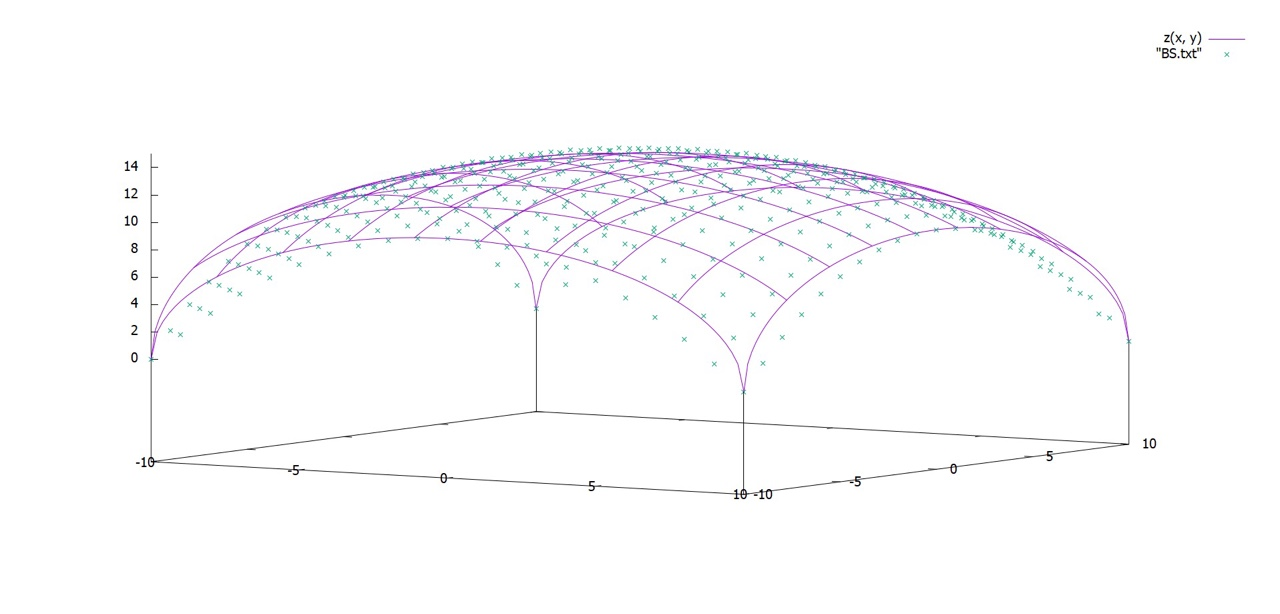
\includegraphics[width=\textwidth]{image/leastSquare}
	\end{center} \setstretch{1.2}
	\caption{$\mathbf{b}_{11}$을 구하는 방법을 적용한 예시}
	\raggedright \small 함수 $z = \sqrt{200 - x^2 - y^2}$의 그래프에 $\mathbf{b}_{11}$을 찾는 방법을 적용한 결과이다. $\mathbf{P}_k$는 $(x, y)$가 $((2i-9)/10, \, (2j-9)/10) \ (i, j = 0, 1, \cdots, 9)$인 점이다. 베지어 곡면과 정점들 사이의 하우스도르프 거리는 약 6.32이다. 
\end{figure}
\begin{figure}[h]
	\begin{center}
		\begin{subfigure}{.2\textwidth}
			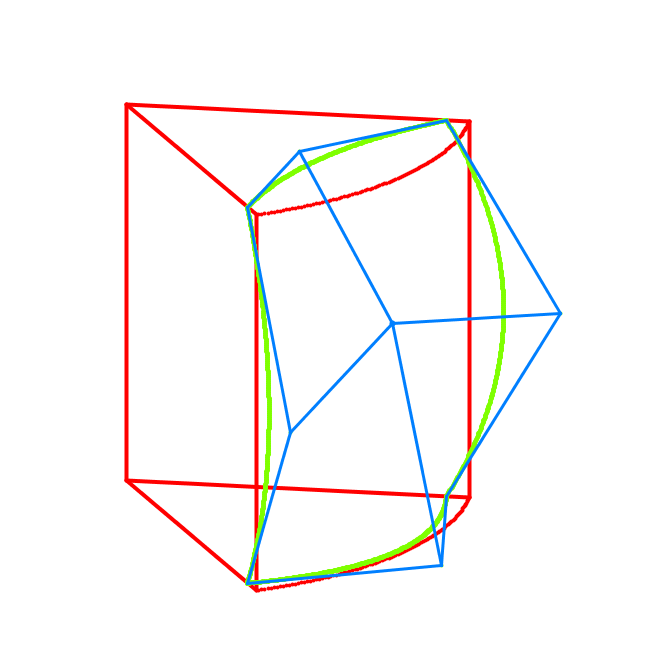
\includegraphics[width=\textwidth]{image/approx3}
		\end{subfigure}
		\begin{subfigure}{.2\textwidth}
			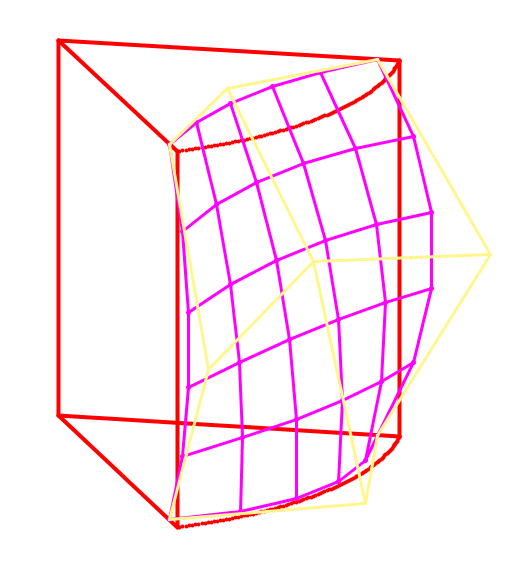
\includegraphics[width=\textwidth]{image/approx4}
		\end{subfigure}
	\end{center} \setstretch{1.2}
	\caption{조절점 - $\mathbf{b}_{11}$}
	\raggedright \small  최소제곱법과 가우스-뉴턴 방법을 통해 $\mathbf{b}_{11}$을 구할 수 있다. 
\end{figure}

\begin{figure}[h]
	\centering
	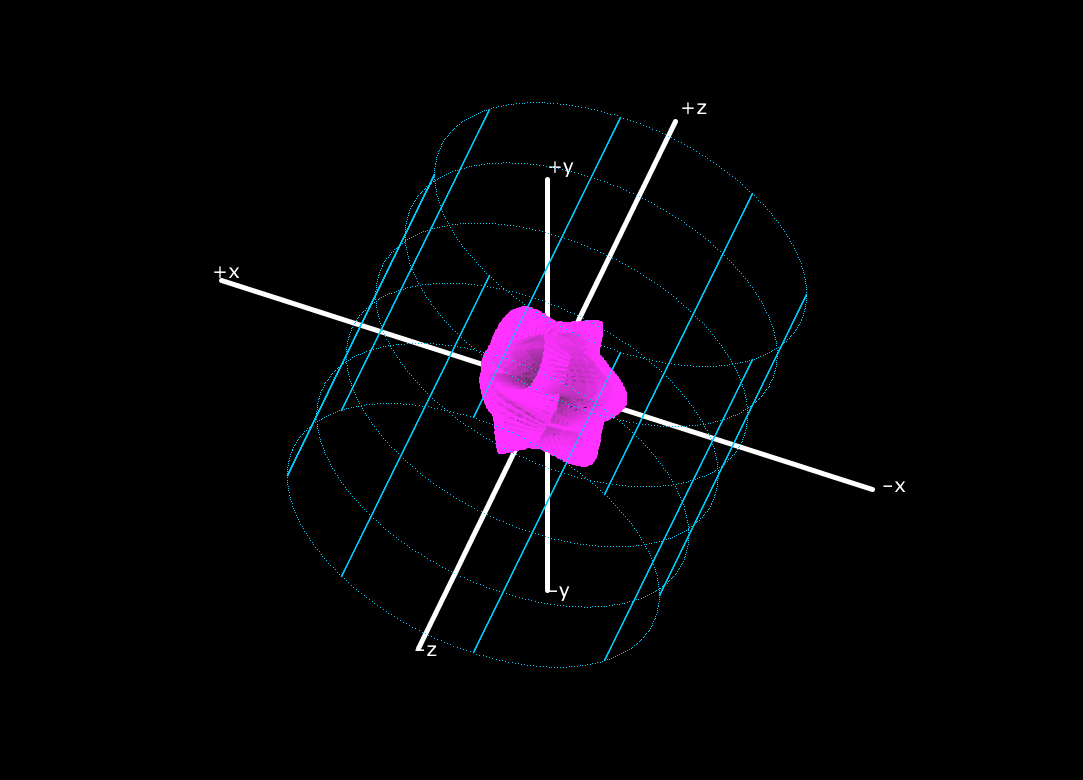
\includegraphics[width=\textwidth]{image/gg}
	\caption{구면 근사}
	\small 반지름 64인 구면은 근사한 모델(분홍색)로, \cref{error}로 정의한 오차함수는 $\mu<10$이다. 
\end{figure}
\subsubsection{수렴성 증명}
\begin{theorem} \label{proj}
	볼록집합 $C \subset \mathbb{R}^3$에 대해 obj파일로 주어진 곡면을 경계 $\partial C$라 하자. 다음과 같이 정의된 함수 $\mathbf{f} \colon [0, 2\pi] \times [-h, h] \to \partial C$는 잘 정의되며, 전사(surjective)이다. 
	$$ \mathbf{f}(\theta_0, z_0) = (\partial C \text{위의 점 중 } \theta = \theta_0, \, z = z_0 \text{인 점}) $$
	(이때 $r=0$인 점은 어떤 $\theta = \theta_0$도 만족한다고 생각한다.)
\end{theorem}
\begin{proof}
	우선 $\partial C$는 닫힌 곡면이므로 정의역의 모든 점이 공역의 적어도 하나의 점에 대응된다는 것은 자명하다. $\mathbf{f}$가 전사임을 보이기 위해 $\partial C$의 모든 점이 $-h \leq z \leq h$ 범위에 있음을 보이면 충분하다. 어떤 점이 $z > h$ 범위에 있다고 가정하자. $\partial C$는 $\mathbf{P}_k$를 꼭짓점으로 하는 다각형 면들의 합집합이므로, 적어도 하나의 정점 $\mathbf{P}_k$가 $z > h$ 범위에 존재해야 한다. 그런데 이는 거리가 가장 먼 두 점이 $(0, 0, \pm h)$라는 사실에 모순이다. 
	
	$(0, 0, \pm h)^\intercal$은 $\partial C$ 위의 점이므로 $\bar{C}$의 원소이다. 보조정리 \ref{closureofconvexset}에 의해 $\bar{C}$는 볼록집합이고, 따라서 $\mathbf{0} \in \bar{C}$이다. 여기서 우리는 각진 모형이 아닌 부드러운 곡면에 대한 근사에 대해서 다루고 있으므로 $\mathbf{0} \in C^\circ$라고 가정할 수 있다. 또한 $\{ (0, 0, z)^\intercal \mid -h < z < h \} \subset C^\circ$이다. 
	
	  $(\theta, z) = (\theta_0, z_0)$를 만족하는 서로 다른 두 점이 있다고 가정해 볼 때, $z_0 = \pm h$이면 이에 대응되는 점은 하나뿐이므로 $-h < z_0 < h$이다. $(0, 0, z_0)$는 $C$의 내부에 있고, 이를 기준으로 정리 \ref{homeo}을 사용하면 $\phi$에 의해 두 점이 같은 점으로 사영되므로 모순이 발생한다는 점에서 $\mathbf{f}$는 잘 정의되며 전사함수임을 알 수 있다.
\end{proof}
또한 $\partial C$는 닫힌 곡면이므로 $\mathbf{f}$는 연속함수이다. $\mathbf{f}$가 연속이 아니라면 $\partial C$가 연속적으로 매개화될 수 없고, 곡면이 아니다. 

\begin{theorem} \label{thm2}
	위와 같은 근사 방법에 따라 3D 모델을 근사했다고 하자. 식 \eqref{error2}로 주어진 오차함수 $\mu$에 대해 다음이 성립한다.
	\begin{equation*}
		\lim_{n\to\infty}\mu=0
	\end{equation*}
\end{theorem} 
\begin{proof}
	$B_i^2(u) B_j^2(v)$의 합이 1이므로 다음이 성립한다.
	\begin{align*}
		\Vert \mathbf{x}_k - \mathbf{P}_k \Vert &= \left\Vert \sum_{i, j = 0}^2 B_i^2(u_k) B_j^2(v_k) (\mathbf{b}_{ij} - \mathbf{P}_k) \right\Vert \\
		&\leq \sum_{i, j = 0}^2 B_i^2(u_k) B_j^2(v_k) \Vert \mathbf{b}_{ij} - \mathbf{P}_k \Vert 
	\end{align*}
	$\Vert \mathbf{x}_k - \mathbf{P}_k \Vert$는 $\Vert \mathbf{b}_{ij} - \mathbf{P}_k \Vert$의 가중평균이므로, $\Vert \mathbf{b}_{ij} - \mathbf{P}_k \Vert \to 0$이면 $\Vert \mathbf{x}_k - \mathbf{P}_k \Vert \to 0$이다. 
	
	정리 \ref{proj}의 함수 $\mathbf{f}$를 생각하자. $\mathbf{f} \colon [0, 2\pi] \times [-h, h] \to \mathbb{R}^3$는 콤팩트 집합에서 정의된 연속함수이므로 Heine-Cantor Theorem에 의해 균등연속(uniformly continuous)이다. 즉, 임의의 $\epsilon > 0$에 대해 다음을 만족하는 $\delta > 0$이 존재한다. 
	$$ \sqrt{(\theta - \theta^\prime)^2 + (z - z^\prime)^2} < \delta \implies \Vert \mathbf{f}(\theta, z) - \mathbf{f}(\theta^\prime, z^\prime) \Vert < \epsilon $$
	
	이제 $\mathbf{P}_k = \mathbf{f}(\theta_k, z_k)$라 하고, $(\theta_k, z_k)$를 포함하는 영역 $$ I_{ab} = \left[ \frac{2\pi a}{2^n}, \, \frac{2\pi(a+1)}{2^n}\right] \times \left[ -h + \frac{2hb}{2^n}, \, -h + \frac{2h(b+1)}{2^n} \right] $$가 $(\theta_k, z_k)$의 $\delta/2$-근방에 포함되도록 하는 최소의 자연수 $N$을 선택하자. $\mathbf{b}_{00}, \mathbf{b}_{02}, \mathbf{b}_{20}, \mathbf{b}_{22} \in \mathbf{f}(I_{ab})$이므로, $n \geq N$이면 $\Vert \mathbf{b}_{00} - \mathbf{P}_k \Vert, \, \Vert \mathbf{b}_{02} - \mathbf{P}_k \Vert, \, \Vert \mathbf{b}_{20} - \mathbf{P}_k \Vert, \, \Vert \mathbf{b}_{22} - \mathbf{P}_k \Vert $는 모두 $\epsilon$ 보다 작다. 또한 $\mathbf{f}(I_{ab})$가 $\mathbf{b}_{00}$의 $\epsilon$-근방에 포함되므로 $\Vert \mathbf{b}_{01} - \mathbf{P}_k \Vert < \Vert \mathbf{b}_{01} - \mathbf{Q} \Vert + \Vert \mathbf{Q} - \mathbf{P}_k \Vert < 2\epsilon$이 성립한다 ($\mathbf{Q}$는 \cref{BCmiddle} 참고). 마찬가지로 $\Vert \mathbf{b}_{01} - \mathbf{P}_k \Vert, \, \Vert \mathbf{b}_{10} - \mathbf{P}_k \Vert, \, \Vert \mathbf{b}_{12} - \mathbf{P}_k \Vert, \, \Vert \mathbf{b}_{21} - \mathbf{P}_k \Vert $는 모두 $2\epsilon$보다 작다. 따라서 $(i, j) \neq (1, 1)$에 대해 $\lim_{n \to \infty} \Vert \mathbf{b}_{ij} - \mathbf{P}_k \Vert = 0$이다. 
	
	$\mathbf{b}_{11}$은 \eqref{secondfindb11}과 같이 주어지고, 이때 $\mathbf{y}_k$는 다음과 같다.
	$$ \mathbf{y}_k = \sum_{(i, j) \neq (1, 1)} B_i^2(u_k) B_j^2(v_k) \mathbf{b}_{ij} $$ $\Vert \mathbf{b}_{11} - \mathbf{P}_k \Vert$는 아래과 같은 부등식으로 계산된다. 
	\begin{align*}
		&\Vert \mathbf{b}_{11} - \mathbf{P}_k \Vert \\
		&= \left\Vert \frac{\sum_{k=1}^K B_1^2(u_k) B_1^2(v_k) \sum_{(i, j) \neq (1, 1)} B_i^2(u_k) B_j^2(v_k) (\mathbf{P}_k - \mathbf{b}_{ij})}{\sum_{k=1}^K (B_1^2(u_k) B_1^2(v_k))^2} \right\Vert \\
		&\leq \frac{\sum_{k=1}^K B_1^2(u_k) B_1^2(v_k) \sum_{(i, j) \neq (1, 1)} B_i^2(u_k) B_j^2(v_k) \Vert \mathbf{P}_k - \mathbf{b}_{ij} \Vert}{\sum_{k=1}^K (B_1^2(u_k) B_1^2(v_k))^2} \\
		&\leq \frac{\sum_{k=1}^K B_1^2(u_k) B_1^2(v_k) (1 - B_1^2(u_k) B_1^2(v_k))}{\sum_{k=1}^K (B_1^2(u_k) B_1^2(v_k))^2} \cdot 2\epsilon
	\end{align*}
    \begin{align*}
		&= \left[ \frac{\sum_{k=1}^K B_1^2(u_k) B_1^2(v_k)}{\sum_{k=1}^K (B_1^2(u_k) B_1^2(v_k))^2} - 1 \right] \cdot 2\epsilon \\
		&\leq \frac{K}{\sum_{k=1}^K (B_1^2(u_k) B_1^2(v_k))^2} \frac\epsilon2
	\end{align*}
	
	마지막 식에서 다음과 같은 절대부등식을 사용했다.
	$$ \frac{\sum_{k=1}^K x_k}{\sum_{k=1}^K x_k^2} \leq 1 + \frac{K}{4\sum_{k=1}^K x_k^2} $$
	이는 절대부등식 $x_k \leq x_k^2 + 1/4$를 변변이 더하고 $\sum x_k^2$으로 나누면 얻을 수 있다. 
	
	$u_k$와 $v_k$가 항상 $[0.01, \, 0.99]$ 범위에 있으므로 $(B_1^2(u_k) B_1^2(v_k))^2 \geq (2 \times 0.01 \times 0.99)^4 = C$이고, 이에 따라 $\Vert \mathbf{b}_{11} - \mathbf{P}_k \Vert \leq \epsilon K / 2C$이다. 여기서 $K$는 영역 안에 있는 점의 개수이다. 전체 점 개수를 $K_{1}$라 한다면  $\Vert \mathbf{b}_{11} - \mathbf{P}_k \Vert \leq \epsilon K / 2C \leq \epsilon K_{1} / 2C$임을 알 수 있다. 모든 $0 \leq i, j \leq 2$에 대해 $\lim_{n \to \infty} \Vert \mathbf{b}_{ij} - \mathbf{P}_k \Vert = 0$이므로, 이들의 가중평균인 $\mathbf{x}_k - \mathbf{P}_k$도 $n \to \infty$의 극한에서 $0$으로 수렴한다. 
	
	각 $k$에 대해서 $\lim_{n \to \infty} \Vert \mathbf{x}_k - \mathbf{P}_k \Vert = 0$이므로, 모든 $\epsilon > 0$에 대해 적당한 자연수 $N_k$가 존재해 $n \geq N_k \implies \Vert \mathbf{x}_k - \mathbf{P}_k \Vert < \epsilon$을 만족한다. 이제 자연수 $N$을 $N_k$들의 최댓값으로 정의한다. 
	$$ N = \max_{\text{각 영역}} \max_{1 \leq k \leq K} N_k $$
	그러면 모든 $n \geq N$에 대해 $\mu < \epsilon$이므로, $\lim_{n \to \infty} \mu = 0$을 얻는다. 
\end{proof}
정리 \ref{thm2}는 제시한 근사 방법에 따라 obj파일로 주어진 곡면을 원하는 오차 범위 내에서 베지어 곡면으로 근사할 수 있음을 의미한다. \\
\subsection{2D model RGB implementation}
이제 각각 모델이 근사가 된다는 것을 보였으니 실생활에 더 넓게 활용될 수 있도록 RGB 근사도 다룰 것이다.
\subsubsection{분할 방법}
일단 2D 근사를 해야하는데 2D영역에 각 점에 색깔이 있다. 이를 쉽게 해석하기 위해 본 연구에서는 R,G,B 따로 따로 근사하고 이에 대한 값을 근사해서 더하는 형태로 근사가 진행될 것이다. 그러면 임의의 2D 그림에 대하여 $(x,y)$위치에 따라 각각 R,G,B값을 함수로 나타낼 필요가 생긴다.
\begin{definition}
{
  2D그림에서 $(x,y)$위치에 대응되는 R,G,B값을 각각  $a,b,c$라고 할때 $f_{R},f_{G},f_{B}$함수를 각각 \textbf{R함수, G함수, B함수}라고 하고 다음과 같이 정의한다.
  \begin{equation}
  	a=f_{R}(x,y), b=f_{G}(x,y), c=f_{B}(x,y)
  \end{equation}
  그리고 우리는 이 $f_{R},f_{G},f_{B}$ 함수를 베지어 곡면으로 근사시킨 함수를 $h_{R},h_{G},h_{B}$함수라고 하면 최종적으로 근사한 2D는 3개의 함수를 더하면 나타날 것이다.
}
\end{definition}
지금부터 근사하는 과정은 R함수, G함수, B함수는 똑같이 진행되므로 R함수를 기준으로 설명할 것이다.

여기서 보면 R함수, G함수, B함수는 2개의 독립변수에 의해 값이 나타나지는 양함수이므로 베지어 곡선보다는 베지어 곡면으로 근사하는 것이 옳을 것이다. 그리고 무엇보다 R 함수, G 함수, B 함수의 그래프 개형만 근사하면 되므로 결국 색깔이 없는 베지어 곡면을 근사하는 것과 비슷하게 하면 됨을 의미한다.

그러면 분할하는 방법은 원통형 분할과 비슷하게 다음과 같이 정의한다.
\begin{definition}
	\textbf{2D RGB 분할}은 x,y 하나의 색상을 축으로 하는 3차원 직교좌표계를 기준으로 하며(x,y)로 표현되는 점즐을 x,y에 따라 나눈다. xy평면에 각 점들을 표현하고 각 축을 반으로 분할해서 영역을 $4^{n}$등분하여 영역을 분할하는 방식이다. 
	
	여기서 $x,y$범위는 각각 $0\leq{x}\leq{a},0\leq{y}\leq{b}$이므로 각 RGB분할을 하면 각 영역은 $x_{i}=a/2^{n},y_{i}=b/2^{n}$을 경계로 함을 알 수 있다.
\end{definition}
\begin{figure}[h]
	\centering
	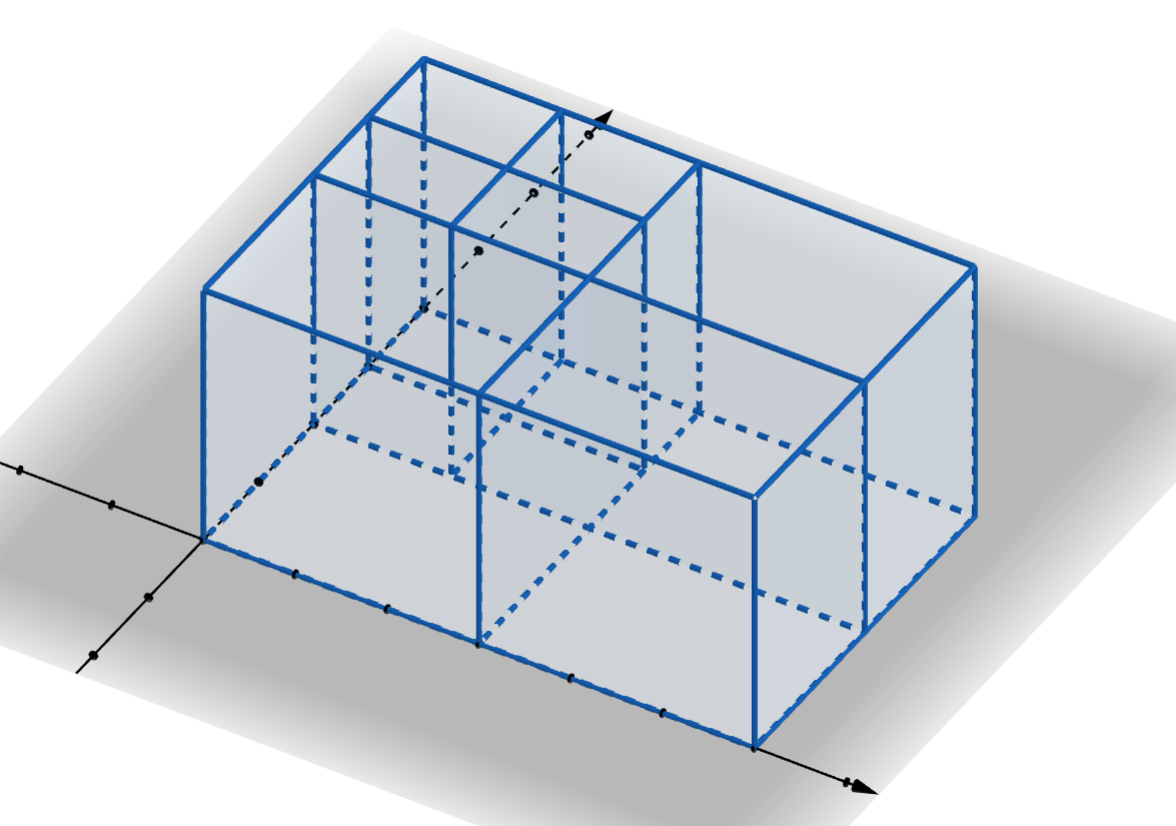
\includegraphics[width=.5\textwidth]{image/RGB2Ddivision}
	\caption{2D RGB 분할}
	\small \raggedright 이 그림에서의 2D RGB 분할은 전반적으로 한번 나누고 그 안에서 오차함수가 기준치보다 높을때 한번더 나뉘어진 모습을 보여주고 있다. 
\end{figure}
\subsubsection{Control Point Determination}
분할된 영역에서  베지어 곡면을 결정하기 위해서는 9개의 점이 필요함을 생각할 수 있다. 
베지어 곡면이 연속적으로 이어지기 위해서는 $\textbf{b}_{11}$를 제외한 나머지 조절점은 영역안에 있는 점들과는 무관하게 결정되어야한다. 각 영역의 경계는 $x=x_{i}$ 혹은 $y=y_{i}$로 주어지므로 직선 $\ell \colon x=x_{i}, y=y_{j}$와 R 함수, G 함수, B 함수의 교점으로 $\textbf{b}_{00},\textbf{b}_{02},\textbf{b}_{20},\textbf{b}_{22}$를 구한다. 여기서 2D모델에서 모든 점에는 색깔이 있으므로 위에서 쓴 Möller-Trumbore intersection algorithm을 사용할 필요는 없다. 그리고 2D model 근사에서 중간 조절점을 잡은 방법을 이용하여 네 조절점 $\textbf{b}_{01},\textbf{b}_{10},\textbf{b}_{12},\textbf{b}_{21}$을 얻을 수 있다. 이는 (2,2)차 베지어 곡면에서 $u=0,u=1,v=0,v=1$인 부분은 2차 베지어 곡선이 되기 때문이다. 이에 대한 그림은 \cref{3D control}에 있으므로 생략하겠다.

$\textbf{b}_{11}$를 구하기 위해 최소제곱법을 이용하였다. 최소제곱법을 사용하기 위해서는 R 함수에서  몇개의 데이터 점 $\textbf{P}_{k}$를 뽑고 이에 대응되는 베지어 곡면위의 점 $\mathbf{x}_k=\mathbf{x}(u_k, v_k)$을 알아야 한다. 이미 알고 있는 8개 조절점에 대한 항을 $\mathbf{y}_k$라 하면 다음과 같이 나타낼 수 있다. 
\begin{equation*}
	\mathbf{x}_k=B_1^2(u_k)B_1^2(v_k)\mathbf{b}_{11}+\mathbf{y}_k
\end{equation*}
이제 $\mathbf{x}_k=\mathbf{P}_k\ (k=1, \cdots, K)$의 제곱오차 $S=\sum_{k=1}^K \| \mathbf{x}_k-\mathbf{P}_k \|^2$를 최소화하기 위해 행렬방정식으로 나타낸다.
\begin{equation*}
	\begin{pmatrix}
		B_1^2(u_1)B_1^2(v_1) \\ B_1^2(u_2)B_1^2(v_2) \\ \vdots \\ B_1^2(u_K)B_1^2(v_K)
	\end{pmatrix} \begin{pmatrix}
		b_{11}^x & b_{11}^y & b_{11}^z
	\end{pmatrix} = \begin{pmatrix}
		P_1^x-y_1^x & P_1^y-y_1^y & P_1^z-y_1^z \\ P_2^x-y_2^x & P_2^y-y_2^y & P_2^z-y_2^z \\ \vdots & \vdots & \vdots \\ P_K^x-y_K^x & P_K^y-y_K^y & P_K^z-y_K^z
	\end{pmatrix}
\end{equation*}
이때 윗첨자 $x, y, z$는 각각 벡터의 $x, y, z$성분을 가르킨다. 이 경우에도 제곱오차는 마찬가지로 $S$이다. $AX=B$ 꼴의 행렬방정식에서 최소제곱오차를 가지는 $\hat{X}$는 $\hat{X}=(A^\intercal A)^{-1}A^\intercal B$로 주어지므로, $\mathbf{b}_{11}$을 다음과 같이 근사할 수 있다. 
\begin{equation} \label{thirdfindb11}
	\mathbf{b}_{11}=\dfrac{\sum_{k=1}^K B_1^2(u_k)B_1^2(v_k)(\mathbf{P}_k-\mathbf{y}_k)}{\sum_{k=1}^K (B_1^2(u_k)B_1^2(v_k))^2}
\end{equation}
각 $k$에 대해 $u_k$와 $v_k$의 값을 안다면 \eqref{thirdfindb11}과 같이 $\mathbf{b}_{11}$을 구할 수 있다. 이제 최적의 $u_k, v_k$를 찾기 위해 뉴턴-랩슨 방법을 이용한다. 뉴턴-랩슨 방법을 적용할 함수는 $\mathbf{x}-\mathbf{P}_k$이다. 즉 현재 $u_{n, k}$와 $v_{n, k}$가 주어질 때, 다음과 같이 $u_{n+1, k}$와 $v_{n+1, k}$를 얻는다. 
\begin{align}
	u_{n+1, k}&=u_{n, k}-\frac{\mathbf{x}-\mathbf{P}_k}{\partial(\mathbf{x}-\mathbf{P}_k)/\partial u} \bigg|_{u=u_{n, k}} \\
	v_{n+1, k}&=v_{n, k}-\frac{\mathbf{x}-\mathbf{P}_k}{\partial(\mathbf{x}-\mathbf{P}_k)/\partial v} \bigg|_{v=v_{n, k}}
\end{align}
그런데 벡터의 나눗셈은 정의되지 않으므로 이번에도 최소제곱법을 이용한다. 즉 $[\partial(\mathbf{x}-\mathbf{P}_k)/\partial u] \Delta u = \mathbf{x}-\mathbf{P}_k$의 제곱 오차를 최소로 하는 스칼라 $\Delta u$를 선택한다.  초기 조건 $u_{0, k}=v_{0, k}=0.5$에 대해 $\mathbf{b}_{11}$를 구하고 새로 $u_k, v_k$를 구하는 과정을 반복한다. 

이번에도 $u_k$와 $v_k$의 값을 거의 일정하게 만들기 위해 위 과정을 20번 반복한다. \\

\subsubsection{Algorithm}
우리는 이제 어떻게 하면 근사가 되는지 살펴볼 것이다. 일단 어떠한 R 함수가 있을때 이를 2D RGB 분할을 할것이다. 그리고 분할된 영역의 곡면을 하나의 베지어 곡면으로 근사를 해볼 것이다. 분할된 영역의 베지어 곡면이 연속적으로 이어지기 위해서는 베지어 곡면의 네 모서리($u=0, \, u=1, \, v=0, \, v=1$)가 영역의 경계에 위치해야 한다. 특히 네 조절점 $\mathbf{b}_{00} = \mathbf{x}(0, 0), \, \mathbf{b}_{02} = \mathbf{x}(0, 1), \, \mathbf{b}_{20} = \mathbf{x}(1, 0), \, \mathbf{b}_{22} = \mathbf{x}(1, 1)$는 각각 4개의 영역이 만나는 경계에 위치한다. 

분할된 영역이 $x_{a} \leq x \leq x_{a+1}, \, y_{b} \leq z \leq y_{b+1}$로 주어진다고 하자. 직선 $\ell_{ab} \colon x = x_{a}, \, y = y_{b}$로 정의하고, 네 직선 $\ell_{ab}, \, \ell_{a, \, b+1}, \, \ell_{a+1, \, b}, \, \ell_{a+1, \, b+1}$과 R함수와의 교점을 찾아 각각 $\mathbf{b}_{00}, \mathbf{b}_{02}, \mathbf{b}_{20}, \mathbf{b}_{22}$로 둔다. 

그리고 점 $(x,y,f_{R})$들 중 $\mathbf{b}_{00}$과 $\mathbf{b}_{02}$를 잇는 직선에서 가장 멀리 떨어진 점 $\mathbf{Q}$를 찾는다. 그러면 $\mathbf{b}_{01} = 2\mathbf{Q} - (\mathbf{b}_{00} + \mathbf{b}_{02})/2$로 주어진다. 같은 방법으로 조절점 $\mathbf{b}_{01}, \mathbf{b}_{10}, \mathbf{b}_{12}, \mathbf{b}_{21}$을 얻을 수 있다. 

이제 조절점 $\mathbf{b}_{11}$을 구하기 위해 최소제곱법과 가우스-뉴턴 방법을 이용한다. 영역 내의 점 $(x,y,f_{R})$을 $\mathbf{P}_k \ (k=1, 2, \cdots, K)$라 하자. 각 $\mathbf{P}_k$에 대응되는 베지어 곡면의 매개변수 $u_k$와 $v_k$가 주어졌다고 가정한다. $\mathbf{x}_k = \mathbf{x}(u_k, v_k)$에서 이미 알고 있는 조절점들에 대한 항을 $\mathbf{y}_k$로 두면 다음과 같이 나타날 수 있다.

$$ \mathbf{x}_k = \mathbf{x}(u_k, v_k) = B_1^2(u_k) B_1^2(v_k) \mathbf{b}_{11} + \mathbf{y}_k $$ 

$\mathbf{b}_{11}$에 관한 연립방정식 $\mathbf{x}_k = \mathbf{P}_k \ (1 \leq k \leq K)$는 일반적으로 해를 가지지 않는다. 따라서 제곱오차 $S = \sum_{k=1}^K \Vert \mathbf{x}_k - \mathbf{P}_k \Vert^2$을 최소로 만드는 $\mathbf{b}_{11}$의 값을 구한다. 이를 위해 $x, y, z$ 좌표로 나눠 행렬방정식으로 표현한다. 
\begin{align*}
	&\begin{pmatrix}
		B_1^2(u_1)B_1^2(v_1) \\ B_1^2(u_2)B_1^2(v_2) \\ \vdots \\ B_1^2(u_K)B_1^2(v_K)
	\end{pmatrix} \begin{pmatrix}
		b_{11}^x & b_{11}^y & b_{11}^z
	\end{pmatrix} 
	= \begin{pmatrix}
		P_1^x-y_1^x & P_1^y-y_1^y & P_1^z-y_1^z \\ P_2^x-y_2^x & P_2^y-y_2^y & P_2^z-y_2^z \\ \vdots & \vdots & \vdots \\ P_K^x-y_K^x & P_K^y-y_K^y & P_K^z-y_K^z
	\end{pmatrix}
\end{align*}
이때 윗첨자 $x, y, z$는 각각 벡터의 $x, y, z$성분을 나타낸다. 위 행렬방정식의 제곱오차도 마찬가지로 $S$임을 알 수 있다. $AX = B$ 꼴의 행렬방정식에서 최소제곱오차를 가지는 $X = (A^\intercal A)^{-1} A^\intercal B$로 주어지므로, 다음과 같이 $\mathbf{b}_{11}$을 구할 수 있다. 
\begin{equation} \label{forthfindb11}
	\mathbf{b}_{11} = \frac{\sum_{k=1}^K B_1^2(u_k) B_1^2 (v_k) (\mathbf{P}_k - \mathbf{y}_k)}{\sum_{k=1}^K (B_1^2(u_k) B_1^2(v_k))^2}
\end{equation}
각 $\mathbf{P}_k$에 대해 대응되는 $u_k$와 $v_k$를 알고 있다면 \eqref{forthfindb11}과 같이 $\mathbf{b}_{11}$을 구할 수 있다. 이제 최적의 $u_k$와 $v_k$를 얻기 위해 가우스-뉴턴 방법을 사용한다. 즉, 각각의 $k$에 대해 $\mathbf{x}_k$와 $\mathbf{P}_k$의 차이를 줄이는 방향으로 $u_k$와 $v_k$를 갱신한다. 현재 $u_{n, \, k}$와 $v_{n, \, k}$의 값이 $\mathbf{u}_{n, \, k} = (u_{n, \, k}, v_{n, \, k})^\intercal$로 주어질 때, 다음과 같이 $\mathbf{u}_{n+1, \, k}$를 알 수 있다. 
\begin{equation} \label{rearrange2}
	\mathbf{u}_{n+1, \, k} = \mathbf{u}_{n, \, k} - (\mathbf{J}_\mathbf{x}^\intercal \mathbf{J}_\mathbf{x})^{-1} \mathbf{J}_\mathbf{x}^\intercal (\mathbf{x}_k - \mathbf{P}_k)
\end{equation}
이때 $\mathbf{J}_\mathbf{x}$는 $\mathbf{u} = (u, v)^\intercal$에 대한 $\mathbf{x}$의 Jacobian matrix이다.

$$ \mathbf{J}_\mathbf{x} = \begin{pmatrix} \partial x^x / \partial u & \partial x^x / \partial v \\ \partial x^y / \partial u & \partial x^y / \partial v \\ \partial x^z / \partial u & \partial x^z / \partial v \end{pmatrix} $$ 

앞에서와 마찬가지로 윗첨자는 벡터의 성분을 나타낸다.

초기조건 $u_{0, \, k} = v_{0, \, k} = 0.5$에 대해, 다음 과정을 3D 모델 근사 부분처럼 반복한다. 
\begin{enumerate}
	\item 식 \eqref{forthfindb11}와 같이 $\mathbf{b}_{11}$을 구한다. 
	\item 식 \eqref{rearrange2}와 같이 $u_k, v_k$를 갱신한다. 
\end{enumerate}

이때, 베지어 곡면은 $0 \leq u, v \leq 1$의 범위에서 정의되므로 중간 과정에서 수렴성을 보장하기 위해 위와 비슷하게 $u_{n, \, k}$ 또는 $v_{n, \, k}$가 0.01보다 작아지면 0.01로 대체하고, 0.99보다 커지면 0.99로 대체한다. 

위의 과정은 3D 모델 근사부분과 동일하다고 할 수 있다 하지만 위의 과정을 R함수 뿐만이 아닌 G,B함수에서도 해야하는 것과 오차함수 부분은 색상까지 표현하는 만큼 다르게 정의해야 한다.
\begin{definition}
	2D RGB저장 부분에서 근사시킨 R,G,B 함수를 각각 $\mathbf{Rx}_k,\mathbf{Gx}_k,\mathbf{Bx}_k$, 근사시키고 싶은 3D 모델에서 뽑은 점들의 R,G,B함수를 각각 $\mathbf{RP}_k,\mathbf{GP}_k,\mathbf{BP}_k$라고 할 때, R오차함수, G오차함수, B오차함수 $\mu_{R},\mu_{G},\mu_{B}$ 와 오차함수 $\mu$는 다음과 같이 주어진다.
	\begin{equation} \label{2D RGB error}
		\begin{split}
		&\mu_{R}=\max_{\text{$f_{R}$ 영역}}\max_{1\leq k\leq K} \| \mathbf{Rx}_k-\mathbf{RP}_k\| \\
		&\mu_{G}=\max_{\text{$f_{G}$ 영역}}\max_{1\leq k\leq K} \| \mathbf{Gx}_k-\mathbf{GP}_k\| \\
		&\mu_{B}=\max_{\text{$f_{B}$ 영역}}\max_{1\leq k\leq K} \| \mathbf{Bx}_k-\mathbf{BP}_k\| \\
		&\mu=\mu_{R}+\mu_{G}+\mu_{B}
		\end{split}
	\end{equation}
\end{definition}


우리는 R 함수, G 함수,B 함수의 분할횟수 중 최솟값을 $n$이라고 하였을때 $n\to\infty$에 따라 $\mu\to0$임을 보였다. 

\subsubsection{수렴성 증명}
\begin{theorem} \label{thm1}
	위와 같은 근사 방법에 따라 $f_{R}$을 근사했다고 하자. 오차함수 $\mu_{R}$에 대해 다음이 성립한다.
	\begin{equation*}
		\lim_{n\to\infty}\mu_{R}=0
	\end{equation*}
\end{theorem} 
\begin{proof}
	$B_i^2(u) B_j^2(v)$의 합이 1이므로 다음이 성립한다.
	\begin{align*}
		\Vert \mathbf{Rx}_k - \mathbf{RP}_k \Vert &= \left\Vert \sum_{i, j = 0}^2 B_i^2(u_k) B_j^2(v_k) (\mathbf{b}_{ij} - \mathbf{RP}_k) \right\Vert \\
		&\leq \sum_{i, j = 0}^2 B_i^2(u_k) B_j^2(v_k) \Vert \mathbf{b}_{ij} - \mathbf{RP}_k \Vert 
	\end{align*}
	$\Vert \mathbf{x}_k - \mathbf{RP}_k \Vert$는 $\Vert \mathbf{b}_{ij} - \mathbf{RP}_k \Vert$의 가중평균이므로, $\Vert \mathbf{b}_{ij} - \mathbf{RP}_k \Vert \to 0$이면 $\Vert \mathbf{x}_k - \mathbf{RP}_k \Vert \to 0$이다. 
	
	 여기서 $f_{R}$은 2개의 독립변수 (x,y)에서 R의 색깔을 반환하는 함수이므로 $\mathbf{f} \colon [0, a] \times [0, b] \to [0,255]$라고 할 수 있고 이는 즉, 콤팩트 집합에서 정의된 연속함수이므로 Heine-Cantor Theorem에 의해 균등연속(uniformly continuous)이다. 임의의 $\epsilon > 0$에 대해 다음을 만족하는 $\delta > 0$이 존재한다. 

	$$ \sqrt{(x - x^\prime)^2 + (y - y^\prime)^2} < \delta \implies \Vert \mathbf{f}_{R}(x,y) - \mathbf{f}_{R}(x^\prime,y^\prime) \Vert < \epsilon $$
	
	이제 $\mathbf{RP}_k = \mathbf{f}_{R}(x_{k},y_{k})$라 하고, $(x,y)$를 포함하는 영역 $$ I_{ab} = \left[ \frac{a}{2^n}, \, \frac{(a+1)}{2^n}\right] \times \left[\frac{b}{2^n}, \,\frac{b+1}{2^n} \right] $$가 $(x,y)$의 $\delta/2$-근방에 포함되도록 하는 최소의 자연수 $N$을 잡자. $\mathbf{b}_{00}, \mathbf{b}_{02}, \mathbf{b}_{20}, \mathbf{b}_{22} \in \mathbf{f}(I_{ab})$이므로, $n \geq N$이면 $\Vert \mathbf{b}_{00} - \mathbf{RP}_k \Vert, \, \Vert \mathbf{b}_{02} - \mathbf{RP}_k \Vert, \, \Vert \mathbf{b}_{20} - \mathbf{RP}_k \Vert, \, \Vert \mathbf{b}_{22} - \mathbf{RP}_k \Vert$는 모두 $\epsilon$보다 작다. 또한 $\mathbf{f}(I_{ab})$가 $\mathbf{b}_{00}$의 $\epsilon$-근방에 포함되므로 $\Vert \mathbf{b}_{01} - \mathbf{RP}_k \Vert < \Vert \mathbf{b}_{01} - \mathbf{Q} \Vert + \Vert \mathbf{Q} - \mathbf{RP}_k \Vert < 2\epsilon$이 성립한다. 마찬가지로 $\Vert \mathbf{b}_{01} - \mathbf{RP}_k \Vert, \, \Vert \mathbf{b}_{10} - \mathbf{RP}_k \Vert, \, \Vert \mathbf{b}_{12} - \mathbf{RP}_k \Vert, \, \Vert \mathbf{b}_{21} - \mathbf{RP}_k \Vert$는 모두 $2\epsilon$보다 작다. 따라서 $(i, j) \neq (1, 1)$에 대해 $\lim_{n \to \infty} \Vert \mathbf{b}_{ij} - \mathbf{RP}_k \Vert = 0$이다. 
	
	$\mathbf{b}_{11}$은 \eqref{forthfindb11}과 같이 주어지고, 이때 $\mathbf{y}_k$는 다음과 같다.
	$$ \mathbf{y}_k = \sum_{(i, j) \neq (1, 1)} B_i^2(u_k) B_j^2(v_k) \mathbf{b}_{ij} $$ $\Vert \mathbf{b}_{11} - \mathbf{RP}_k \Vert$는 아래과 같은 부등식으로 계산된다. 
	\begin{align*}
		&\Vert \mathbf{b}_{11} - \mathbf{RP}_k \Vert \\
		&= \left\Vert \frac{\sum_{k=1}^K B_1^2(u_k) B_1^2(v_k) \sum_{(i, j) \neq (1, 1)} B_i^2(u_k) B_j^2(v_k) (\mathbf{RP}_k - \mathbf{b}_{ij})}{\sum_{k=1}^K (B_1^2(u_k) B_1^2(v_k))^2} \right\Vert \\
		&\leq \frac{\sum_{k=1}^K B_1^2(u_k) B_1^2(v_k) \sum_{(i, j) \neq (1, 1)} B_i^2(u_k) B_j^2(v_k) \Vert \mathbf{RP}_k - \mathbf{b}_{ij} \Vert}{\sum_{k=1}^K (B_1^2(u_k) B_1^2(v_k))^2} \\
		&\leq \frac{\sum_{k=1}^K B_1^2(u_k) B_1^2(v_k) (1 - B_1^2(u_k) B_1^2(v_k))}{\sum_{k=1}^K (B_1^2(u_k) B_1^2(v_k))^2} \cdot 2\epsilon \\
		&= \left[ \frac{\sum_{k=1}^K B_1^2(u_k) B_1^2(v_k)}{\sum_{k=1}^K (B_1^2(u_k) B_1^2(v_k))^2} - 1 \right] \cdot 2\epsilon \\
		&\leq \frac{K}{\sum_{k=1}^K (B_1^2(u_k) B_1^2(v_k))^2} \frac\epsilon2
	\end{align*}
	
	마지막 식에서 다음과 같은 절대부등식을 사용했다.
	$$ \frac{\sum_{k=1}^K x_k}{\sum_{k=1}^K x_k^2} \leq 1 + \frac{K}{4\sum_{k=1}^K x_k^2} $$
	이는 절대부등식 $x_k \leq x_k^2 + 1/4$를 변변이 더하고 $\sum x_k^2$으로 나누면 얻을 수 있다. 
	
	$u_k$와 $v_k$가 항상 $[0.01, \, 0.99]$ 범위에 있으므로 $(B_1^2(u_k) B_1^2(v_k))^2 \geq (2 \times 0.01 \times 0.99)^4 = C$이고, 이에 따라 $\Vert \mathbf{b}_{11} - \mathbf{RP}_k \Vert \leq \epsilon K / 2C$이다. 여기서 $K$는 영역 안에 있는 점의 개수이다. 전체 점 개수를 $K_{1}$라 한다면  $\Vert \mathbf{b}_{11} - \mathbf{RP}_k \Vert \leq \epsilon K / 2C \leq \epsilon K_{1} / 2C$임을 알 수 있다. 모든 $0 \leq i, j \leq 2$에 대해 $\lim_{n \to \infty} \Vert \mathbf{b}_{ij} - \mathbf{RP}_k \Vert = 0$이므로, 이들의 가중평균인 $\mathbf{x}_k - \mathbf{RP}_k$도 $n \to \infty$의 극한에서 $0$으로 수렴한다. 
	
	각 $k$에 대해서 $\lim_{n \to \infty} \Vert \mathbf{x}_k - \mathbf{RP}_k \Vert = 0$이므로, 모든 $\epsilon > 0$에 대해 적당한 자연수 $N_k$가 존재해 $n \geq N_k \implies \Vert \mathbf{x}_k - \mathbf{RP}_k \Vert < \epsilon_{R}$을 만족한다. 이제 자연수 $N_{R}$을 $N_k$들의 최댓값으로 정의한다. 
	$$ N_{R} = \max_{\text{각 영역}} \max_{1 \leq k \leq K} N_k $$
	그러면 모든 $n \geq N_{R}$에 대해 $\mu < \epsilon_{R}$이므로, $\lim_{n \to \infty} \mu_{R} = 0$을 얻는다. 
\end{proof}
우리는 정리 \ref{thm1}에 따라 다음을 얻을 수 있다.
\begin{theorem}
	우리가 R함수, G함수, B함수를 위와 같이 근사했다고 가정하자. 그러면 오차함수 $\mu$에 대해서 다음이 성립한다. 
	\begin{equation*}
		\lim_{n\to\infty}\mu=0
	\end{equation*}
\end{theorem}
\begin{proof}
	우리는 오차함수 $\mu$를 다음과 같이 정의했었다. 
		\begin{equation*}
		 \mu=\mu_{R}+\mu_{G}+\mu_{B}
	    \end{equation*}
    근데 우리는 $\mu_{R}$이 0으로 수렴함을 증명하였다. 비슷하게 $\mu_{G},\mu_{B}$도 0으로 수렴함을 알 수 있으므로 $\mu$도 수렴함을 알 수 있다.
\end{proof}
이 과정을 통해 우리는 분할 횟수를 늘릴때 항상 오차함수가 0으로 수렴함을 보일 수 있었다.
\subsection{3D model RGB implementation}
2차원에서 색상이 있을때 근사하는 방법을 알아보았다면 이번에는 3차원에서 색상이 있을때 근사하는 방법을 알아볼 것이다. 2차원일때는 이에 해당되는 R,G,B 값을 하나의 축으로 하여 3차원 그래프 상에서 근사하였다면 이번에는 약간 다르게 새로운 벡터를 정의하고 그것을 3차원 모델 근사처럼 비슷하게 가져갈 것이다
\begin{definition}
	만약 점 $\textbf{P}$에 색상벡터 $\textbf{Q}$가 대응된다면 우리는 $\textbf{P}$,$\textbf{Q}$ 순서대로 열에 배열한 벡터 $\textbf{K}$를 \textbf{색상 위치 벡터}라고 정의한다.
\end{definition}
즉 우리는 색상 위치 벡터들의 모임을 가중치 베지어 곡면을 이용하여 근사할 것이다. 
위의 근사 방법과 약간 다른 점은 위치 벡터가 색상 위치 벡터인 것이고 베지어 곡면으로 근사하는 대신 가중치 베지어 곡면으로 근사한다는 것이다. 
이러한 점에서 분할하는 방법은 가장 거리가 먼 2개의 점을 z축에 배치하고 원통형 분할을 하던 것 그대로 가져갈 것이다. 하지만 가중치 베지어 곡면의 RGB 조절점에 대한 것은 약간 다른 점이 있어 조절점을 정하는 방법을 알아볼 것이다.

\subsubsection{Control Point Determination}
이제 원통형 분할로 나뉘어진 영역에 존재하는 색상 위치 벡터를 (2,2)차 가중치 베지어 곡면으로 근사해야 한다. 가중치 베지어 곡면을 결정하기 위해서는 RGB 조절점 9개를 잡아야한다. 일단 가중치 베지어 곡면이 연속적으로 이어지기 위해서는 $\mathbf{k}_{11}$를 제외한 나머지 조절점은 영역 안에 있는 정점들과는 무관하게 결정되어야 한다. 각 영역의 경계는 $\theta=\theta_i$ 혹은 $z=z_j$로 주어지므로, 직선 $\ell \colon \theta=\theta_i, z=z_j$와 obj 파일의 면 $F$의 교점으로 네 조절점 $\mathbf{k}_{00}, \mathbf{k}_{02}, \mathbf{k}_{20}, \mathbf{k}_{22}$를 구한다. 여기서는 직선과 삼각형의 교점을 찾는 빠른 알고리즘인 Möller-Trumbore intersection algorithm을 사용한다. 그리고 여기서 이 알고리즘은 교점을 얻을 수 있는 알고리즘이지만 이 알고리즘에 있는 위치벡터를 색상위치 벡터로 바꿔준다면 교점이 색상 위치 벡터 꼴로 나와 우리는 이 한계점을 극복할 수 있다.\cite{raytriangle} 우리는 2D model 근사에서 중간 조절점을 잡은 방법을 이용하여 네 조절점 $\mathbf{k}_{01}, \mathbf{k}_{10}, \mathbf{k}_{12}, \mathbf{k}_{21}$을 얻을 수 있다. 여기서 색상벡터도 결국 2차 베지어 곡선을 따르므로 중간 조절점을 얻는 방법을 가중치 베지어 곡선에 적용하여 색상조절점 벡터을 이용하여 구해도 무관하다. 이에 대한 그림은 앞에서와 같이 \cref{3D control}부분에 있으므로 생략한다.

$\mathbf{k}_{11}$을 구하기 위해 최소제곱법을 이용한다. 
최소제곱법을 사용하기 위해서는 obj,mtl 파일의 각 색상 위치 벡터 $\mathbf{P}_k$에 대응되는 가중치 베지어 곡면 위의 색상위치벡터 $\mathbf{x}_k=\mathbf{x}(u_k, v_k)$을 알아야 한다. 이미 알고 있는 8개 RGB 조절점에 대한 항을 $\mathbf{y}_k$라 하면 다음과 같이 나타낼 수 있다. 
\begin{equation*}
	\mathbf{x}_k=B_1^2(u_k)B_1^2(v_k)\mathbf{k}_{11}+\mathbf{y}_k
\end{equation*}
이제 $\mathbf{x}_k=\mathbf{P}_k\ (k=1, \cdots, K)$의 제곱오차 $S=\sum_{k=1}^K \| \mathbf{x}_k-\mathbf{P}_k \|^2$를 최소화하기 위해 행렬방정식으로 나타낸다.
\begin{equation*}
	\begin{split}
	&\begin{pmatrix}
		B_1^2(u_1)B_1^2(v_1) \\ B_1^2(u_2)B_1^2(v_2) \\ \vdots \\ B_1^2(u_K)B_1^2(v_K) 
	\end{pmatrix} \begin{pmatrix}
		k_{11}^x & k_{11}^y & k_{11}^z & k_{11}^R & k_{11}^G & k_{11}^B
	\end{pmatrix}  \\
    &= \begin{pmatrix}
		P_1^x-y_1^x & P_1^y-y_1^y & P_1^z-y_1^z & P_1^R-y_1^R & P_1^G-y_1^G & P_1^B-y_1^B \\ P_2^x-y_2^x & P_2^y-y_2^y & P_2^z-y_2^z & P_2^R-y_2^R & P_2^G-y_2^G & P_2^B-y_2^B \\ \vdots & \vdots & \vdots & \vdots & \vdots & \vdots\\ 
		P_K^x-y_K^x & P_K^y-y_K^y & P_K^z-y_K^z & P_K^R-y_K^R & P_K^G-y_K^G & P_K^B-y_K^B
	\end{pmatrix}
    \end{split}
\end{equation*}
이때 윗첨자 $x, y, z$는 각각 벡터의 $x, y, z$성분을 가르키고 윗첨자 $R, G, B$는 각각 색상 벡터의 $R, G, B$성분을 가르킨다. 이 경우에도 제곱오차는 마찬가지로 $S$이다. $AX=B$ 꼴의 행렬방정식에서 최소제곱오차를 가지는 $\hat{X}$는 $\hat{X}=(A^\intercal A)^{-1}A^\intercal B$로 주어지므로, $\mathbf{k}_{11}$을 다음과 같이 근사할 수 있다. 
\begin{equation} \label{findb11}
	\mathbf{k}_{11}=\frac{\sum_{k=1}^K B_1^2(u_k)B_1^2(v_k)(\mathbf{P}_k-\mathbf{y}_k)}{\sum_{k=1}^K (B_1^2(u_k)B_1^2(v_k))^2}
\end{equation}
각 $k$에 대해 $u_k$와 $v_k$의 값을 안다면 \cref{findb11}과 같이 $\mathbf{k}_{11}$을 구할 수 있다. 이제 최적의 $u_k, v_k$를 찾기 위해 뉴턴-랩슨 방법을 이용한다. 뉴턴-랩슨 방법을 적용할 함수는 $\mathbf{x}-\mathbf{P}_k$이다. 즉 현재 $u_{n, k}$와 $v_{n, k}$가 주어질 때, 다음과 같이 $u_{n+1, k}$와 $v_{n+1, k}$를 얻는다.
\begin{align} 
	u_{n+1, k}&=u_{n, k}-\frac{\mathbf{x}-\mathbf{P}_k}{\partial(\mathbf{x}-\mathbf{P}_k)/\partial u} \bigg|_{u=u_{n, k}} \\
	v_{n+1, k}&=v_{n, k}-\frac{\mathbf{x}-\mathbf{P}_k}{\partial(\mathbf{x}-\mathbf{P}_k)/\partial v} \bigg|_{v=v_{n, k}} 
\end{align}
그런데 벡터의 나눗셈은 정의되지 않으므로 이번에도 최소제곱법을 이용한다. 즉, $[\partial(\mathbf{x}-\mathbf{P}_k)/\partial u] \Delta u = \mathbf{x}-\mathbf{P}_k$의 제곱 오차를 최소로 하는 스칼라 $\Delta u$를 선택한다. \\

초기 조건 $u_{0, k}=v_{0, k}=0.5$에 대해 $\mathbf{k}_{11}$를 구하고 새로 $u_k, v_k$를 구하는 과정을 반복한다. 

\subsubsection{Algorithm}
일단 어떠한 3D RGB 모델이 있을때 위에서 말했던 것처럼 축을 돌리고 이를 원통형 분할을 할 것이다.
\begin{figure}[h]
	\begin{center}
		\begin{subfigure}{.3\textwidth}
			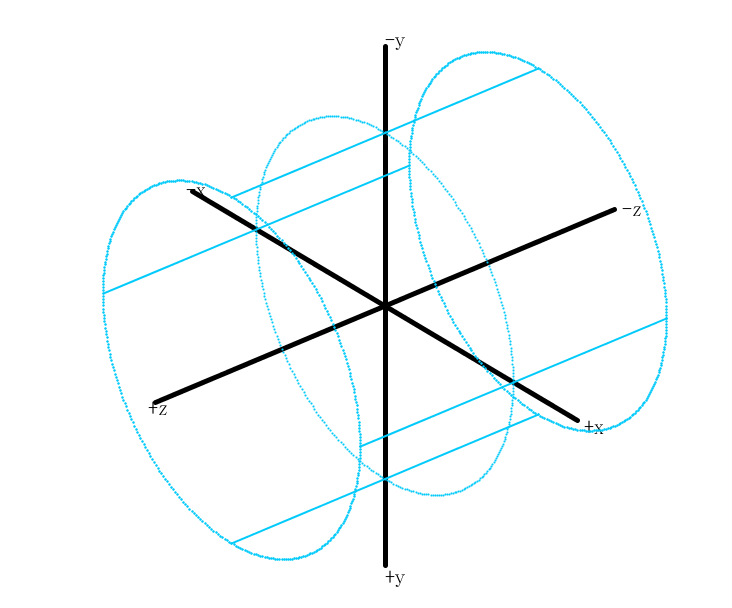
\includegraphics[width=\textwidth]{image/subdivision1}
			\caption{$n=1$}
		\end{subfigure}
		\begin{subfigure}{.3\textwidth}
			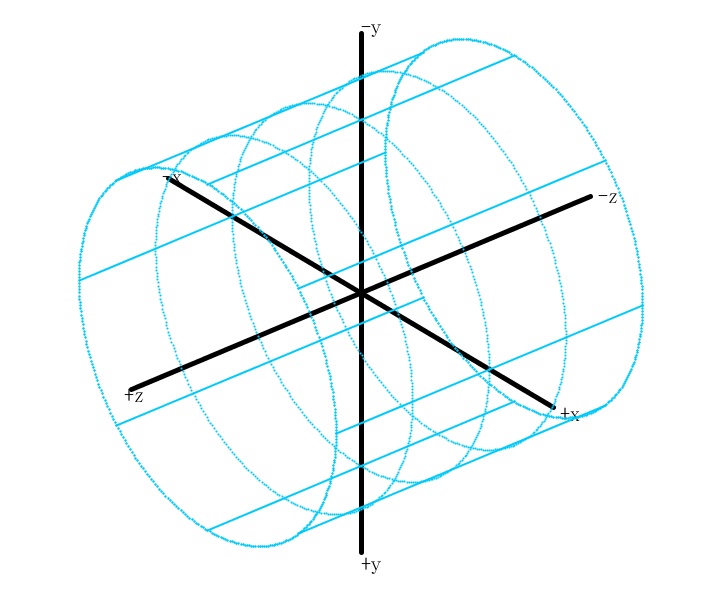
\includegraphics[width=\textwidth]{image/subdivision2}
			\caption{$n=2$}
		\end{subfigure}
		\begin{subfigure}{.3\textwidth}
			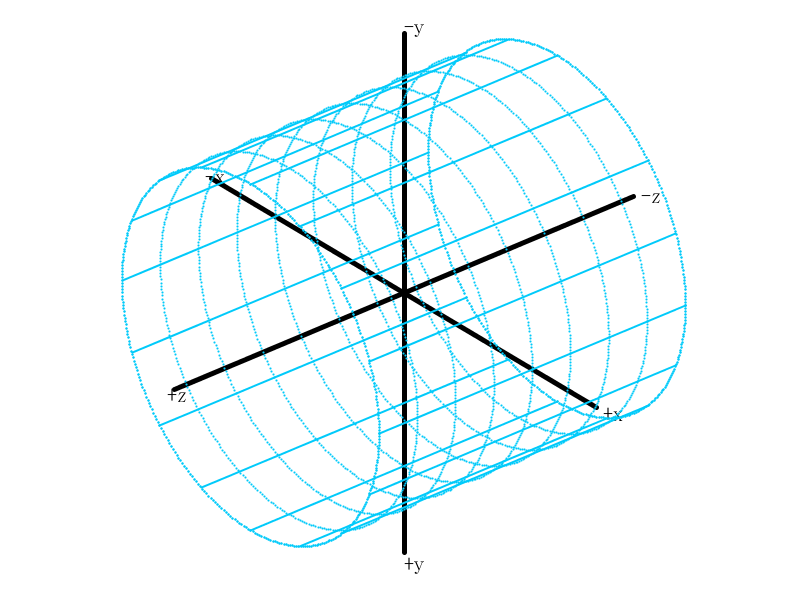
\includegraphics[width=\textwidth]{image/subdivision3}
			\caption{$n=3$}
		\end{subfigure}
	\end{center} \setstretch{1.2}
    \caption{원통형 분할}
	\raggedright \small  원통형 분할은 $\theta$와 $z$의 범위를 이등분하며 이루어진다. 그림에서는 $\theta$와 $z$의 범위를 각각 $2^{n+1}$, $2^n$등분했다. 
\end{figure}

분할된 영역의 곡면을 하나의 가중치 베지어 곡면으로 근사한다. 각 영역의 가중치 베지어 곡면이 연속적으로 이어지기 위해서는 베지어 곡면의 네 모서리($u=0, \, u=1, \, v=0, \, v=1$)가 영역의 경계에 위치해야 한다. 특히 네 RGB 조절점 $\mathbf{k}_{00} = \mathbf{x}(0, 0), \, \mathbf{k}_{02} = \mathbf{x}(0, 1), \, \mathbf{k}_{20} = \mathbf{k}(1, 0), \, \mathbf{k}_{22} = \mathbf{x}(1, 1)$는 각각 4개의 영역이 만나는 경계에 위치한다. 

분할된 영역이 $\theta_a \leq \theta \leq \theta_{a+1}, \, z_b \leq z \leq z_{b+1}$로 주어진다고 하자. 반직선 $\ell_{ab} \colon \theta = \theta_a, \, z = z_b$로 정의하고, 네 반직선 $\ell_{ab}, \, \ell_{a, \, b+1}, \, \ell_{a+1, \, b}, \, \ell_{a+1, \, b+1}$과 obj파일의 면 $F$의 교점을 찾아 각각 $\mathbf{k}_{00}, \mathbf{k}_{02}, \mathbf{k}_{20}, \mathbf{k}_{22}$로 둔다. 이때 광선 또는 직선과 삼각형의 교점을 방법인 Möller-Trumbore intersection algorithm을 이용한다. \cite{raytriangle}

Möller-Trumbore intersection algorithm을 이용하면 영역의 경계 $\theta_a \leq \theta \leq \theta_{a+1}, \, z = z_b$와 $F$의 교선을 찾을 수 있다. 그리고 앞에서 말한 이유 때문에 가중치 베지어 곡선에도  다음 2차 베지어 곡선의 성질\eqref{BCmiddle}을 이용할 수 있었다.

따라서 영역의 경계 $\theta_a \leq \theta \leq \theta_{a+1}, \, z = z_b$와 $\partial C$의 교선을 잡고, 교선 위의 점들 중 $\mathbf{k}_{00}$과 $\mathbf{k}_{02}$를 잇는 직선에서 가장 멀리 떨어진 점에 대응되는 색상 위치 벡터 $\mathbf{Q}$를 찾는다. 그러면 $\mathbf{k}_{01} = 2\mathbf{Q} - (\mathbf{k}_{00} + \mathbf{k}_{02})/2$로 주어진다. 같은 방법으로 조절점 $\mathbf{k}_{01}, \mathbf{k}_{10}, \mathbf{k}_{12}, \mathbf{k}_{21}$을 얻을 수 있다. 

이제 RGB 조절점 $\mathbf{k}_{11}$을 구하기 위해 최소제곱법과 가우스-뉴턴 방법을 이용한다. 이 아이디어는 선형 연구를 참고했다. \cite{2021} 영역 내의 색상 위치 벡터를 $\mathbf{P}_k \ (k=1, 2, \cdots, K)$라 하자. 각 $\mathbf{P}_k$에 대응되는 가중치 베지어 곡면의 매개변수 $u_k$와 $v_k$가 주어졌다고 가정한다. $\mathbf{x}_k = \mathbf{x}(u_k, v_k)$에서 이미 알고 있는 RGB 조절점들에 대한 항을 $\mathbf{y}_k$로 두면 다음과 같이 나타날 수 있다.

$$ \mathbf{x}_k = \mathbf{x}(u_k, v_k) = B_1^2(u_k) B_1^2(v_k) \mathbf{k}_{11} + \mathbf{y}_k $$ 

$\mathbf{k}_{11}$에 관한 연립방정식 $\mathbf{x}_k = \mathbf{P}_k \ (1 \leq k \leq K)$는 일반적으로 해를 가지지 않는다. 따라서 제곱오차 $S = \sum_{k=1}^K \Vert \mathbf{x}_k - \mathbf{P}_k \Vert^2$을 최소로 만드는 $\mathbf{k}_{11}$의 값을 구한다. 이를 위해 $x, y, z, R, G, B$ 좌표로 나눠 행렬방정식으로 표현한다. 
\begin{align*}
	&\begin{pmatrix}
		B_1^2(u_1)B_1^2(v_1) \\ B_1^2(u_2)B_1^2(v_2) \\ \vdots \\ B_1^2(u_K)B_1^2(v_K)
	\end{pmatrix} \begin{pmatrix}
		k_{11}^x & k_{11}^y & k_{11}^z & k_{11}^R & k_{11}^G & k_{11}^B
	\end{pmatrix} \\
	&= \begin{pmatrix}
		P_1^x-y_1^x & P_1^y-y_1^y & P_1^z-y_1^z & P_1^R-y_1^R & P_1^G-y_1^G & P_1^B-y_1^B \\ P_2^x-y_2^x & P_2^y-y_2^y & P_2^z-y_2^z & P_2^R-y_2^R & P_2^G-y_2^G & P_2^B-y_2^B \\ \vdots & \vdots & \vdots & \vdots & \vdots & \vdots\\ 
		P_K^x-y_K^x & P_K^y-y_K^y & P_K^z-y_K^z & P_K^R-y_K^R & P_K^G-y_K^G & P_K^B-y_K^B
		\end{pmatrix}
\end{align*}
이때 윗첨자 $x, y, z$는 각각 벡터의 $x, y, z$성분, $R, G, B$는 각각 색상 벡터의 $R, G, B$성분을 나타낸다. 위 행렬방정식의 제곱오차도 마찬가지로 $S$임을 알 수 있다. $AX = B$ 꼴의 행렬방정식에서 최소제곱오차를 가지는 $X = (A^\intercal A)^{-1} A^\intercal B$로 주어지므로, 다음과 같이 $\mathbf{k}_{11}$을 구할 수 있다. 
\begin{equation} \label{findk11}
	\mathbf{k}_{11} = \frac{\sum_{k=1}^K B_1^2(u_k) B_1^2 (v_k) (\mathbf{P}_k - \mathbf{y}_k)}{\sum_{k=1}^K (B_1^2(u_k) B_1^2(v_k))^2}
\end{equation}
각 $\mathbf{P}_k$에 대해 대응되는 $u_k$와 $v_k$를 알고 있다면 \eqref{findk11}과 같이 $\mathbf{k}_{11}$을 구할 수 있다. 이제 최적의 $u_k$와 $v_k$를 얻기 위해 가우스-뉴턴 방법을 사용한다. 즉, 각각의 $k$에 대해 $\mathbf{x}_k$와 $\mathbf{P}_k$의 차이를 줄이는 방향으로 $u_k$와 $v_k$를 갱신한다. 현재 $u_{n, \, k}$와 $v_{n, \, k}$의 값이 $\mathbf{u}_{n, \, k} = (u_{n, \, k}, v_{n, \, k})^\intercal$로 주어질 때, 다음과 같이 $\mathbf{u}_{n+1, \, k}$를 알 수 있다. 
\begin{equation} 
	\mathbf{u}_{n+1, \, k} = \mathbf{u}_{n, \, k} - (\mathbf{J}_\mathbf{x}^\intercal \mathbf{J}_\mathbf{x})^{-1} \mathbf{J}_\mathbf{x}^\intercal (\mathbf{x}_k - \mathbf{P}_k)
\end{equation}
이때 $\mathbf{J}_\mathbf{x}$는 $\mathbf{u} = (u, v)^\intercal$에 대한 $\mathbf{x}$의 Jacobian matrix이다.

$$ \mathbf{J}_\mathbf{x} = \begin{pmatrix} \partial x^x / \partial u & \partial x^x / \partial v \\ \partial x^y / \partial u & \partial x^y / \partial v \\ \partial x^z / \partial u & \partial x^z / \partial v \\ \partial x^R / \partial u & \partial x^R / \partial v \\ \partial x^G / \partial u & \partial x^G / \partial v \\ \partial x^B / \partial u & \partial x^B / \partial v \end{pmatrix} $$ 

앞에서와 마찬가지로 윗첨자는 벡터의 성분을 나타낸다.

초기조건 $u_{0, \, k} = v_{0, \, k} = 0.5$에 대해, $\mathbf{k}_{11}$를 구하고 $u_k, v_k$를 갱신하는 과정을 반복한다. 

이때, 베지어 곡면은 $0 \leq u, v \leq 1$의 범위에서 정의되므로 중간 과정에서 $u_{n, \, k}$ 또는 $v_{n, \, k}$가 0.01보다 작아지면 0.01로 대체하고, 0.99보다 커지면 0.99로 대체한다. 가우스-뉴턴 방법은 수렴성을 보장할 수 없기 때문에, 이러한 보정은 $u_{n, \, k}$ 또는 $v_{n, \, k}$가 발산하지 않도록 한다.

그러면 이제 가중치 베지어 곡면으로 근사하는 과정을 알아보았으니 새로운 오차함수에 대해 알아보아야 한다.
\begin{definition}
	RGB 저장 부분에서 오차함수는 다음과 같이 정의한다. 분할된 각 영역 내의 색상 위치 벡터를 $\mathbf{P}_k\ (1\leq k\leq K)$라고 하고, 이에 대응되는 가중치 베지어 곡면 위의 색상 위치 벡터를 $\mathbf{x}(u_k, v_k)=\mathbf{x}_k$라 하자. 이때 오차함수 $\mu$는 다음과 같이 주어진다.
	\begin{equation} \label{error}
		\mu=\max_{\text{각 영역}}\max_{1\leq k\leq K} \| \mathbf{x}_k-\mathbf{P}_k \|
	\end{equation}
\end{definition}
우리는 $n\to\infty$에 따라 $\mu\to0$임을 보였다. 
\subsubsection{수렴성 증명}
\begin{theorem} \label{thm}
	위와 같은 근사 방법에 따라 3D 모델을 근사했다고 하자. 식 \eqref{error}로 주어진 오차함수 $\mu$에 대해 다음이 성립한다.
	\begin{equation*}
		\lim_{n\to\infty}\mu=0
	\end{equation*}
\end{theorem} 
\begin{proof}
	$B_i^2(u) B_j^2(v)$의 합이 1이므로 다음이 성립한다.
	\begin{align*}
		\Vert \mathbf{x}_k - \mathbf{P}_k \Vert &= \left\Vert \sum_{i, j = 0}^2 B_i^2(u_k) B_j^2(v_k) (\mathbf{k}_{ij} - \mathbf{P}_k) \right\Vert \\
		&\leq \sum_{i, j = 0}^2 B_i^2(u_k) B_j^2(v_k) \Vert \mathbf{k}_{ij} - \mathbf{P}_k \Vert 
	\end{align*}
	$\Vert \mathbf{x}_k - \mathbf{P}_k \Vert$는 $\Vert \mathbf{k}_{ij} - \mathbf{P}_k \Vert$의 가중평균이므로, $\Vert \mathbf{k}_{ij} - \mathbf{P}_k \Vert \to 0$이면 $\Vert \mathbf{x}_k - \mathbf{P}_k \Vert \to 0$이다. 
	
	정리 \ref{proj}의 함수 $\mathbf{f}$를 생각하자. $\mathbf{f} \colon [0, 2\pi] \times [-h, h] \to \mathbb{R}^3$는 콤팩트 집합에서 정의된 연속함수이므로 Heine-Cantor Theorem에 의해 균등연속(uniformly continuous)이다. 즉, 임의의 $\epsilon > 0$에 대해 다음을 만족하는 $\delta > 0$이 존재한다. 
	$$ \sqrt{(\theta - \theta^\prime)^2 + (z - z^\prime)^2} < \delta \implies \Vert \mathbf{f}(\theta, z) - \mathbf{f}(\theta^\prime, z^\prime) \Vert < \epsilon $$
	
	이제 $\mathbf{P}_k = \mathbf{f}(\theta_k, z_k)$라 하고, $(\theta_k, z_k)$를 포함하는 영역 $$ I_{ab} = \left[ \frac{2\pi a}{2^n}, \, \frac{2\pi(a+1)}{2^n}\right] \times \left[ -h + \frac{2hb}{2^n}, \, -h + \frac{2h(b+1)}{2^n} \right] $$가 $(\theta_k, z_k)$의 $\delta/2$-근방에 포함되도록 하는 최소의 자연수 $N$을 잡자. $\mathbf{k}_{00}, \mathbf{k}_{02}, \mathbf{k}_{20}, \mathbf{k}_{22} \in \mathbf{f}(I_{ab})$이므로, $n \geq N$이면 $\Vert \mathbf{k}_{00} - \mathbf{P}_k \Vert, \, \Vert \mathbf{k}_{02} - \mathbf{P}_k \Vert, \, \Vert \mathbf{k}_{20} - \mathbf{P}_k \Vert, \, \Vert \mathbf{k}_{22} - \mathbf{P}_k \Vert$는 모두 $\epsilon$보다 작다. 또한 $\mathbf{f}(I_{ab})$가 $\mathbf{k}_{00}$의 $\epsilon$-근방에 포함되므로 $\Vert \mathbf{k}_{01} - \mathbf{P}_k \Vert < \Vert \mathbf{k}_{01} - \mathbf{Q} \Vert + \Vert \mathbf{Q} - \mathbf{P}_k \Vert < 2\epsilon$이 성립한다. 마찬가지로 $\Vert \mathbf{k}_{01} - \mathbf{P}_k \Vert, \, \Vert \mathbf{k}_{10} - \mathbf{P}_k \Vert, \, \Vert \mathbf{k}_{12} - \mathbf{P}_k \Vert, \, \Vert \mathbf{k}_{21} - \mathbf{P}_k \Vert$는 모두 $2\epsilon$보다 작다. 따라서 $(i, j) \neq (1, 1)$에 대해 $\lim_{n \to \infty} \Vert \mathbf{k}_{ij} - \mathbf{P}_k \Vert = 0$이다. 
	
	$\mathbf{k}_{11}$은 \eqref{findk11}과 같이 주어지고, 이때 $\mathbf{y}_k$는 다음과 같다.
	$$ \mathbf{y}_k = \sum_{(i, j) \neq (1, 1)} B_i^2(u_k) B_j^2(v_k) \mathbf{k}_{ij} $$ $\Vert \mathbf{k}_{11} - \mathbf{P}_k \Vert$는 아래과 같은 부등식으로 계산된다. 
	\begin{align*}
		&\Vert \mathbf{k}_{11} - \mathbf{P}_k \Vert \\
		&= \left\Vert \frac{\sum_{k=1}^K B_1^2(u_k) B_1^2(v_k) \sum_{(i, j) \neq (1, 1)} B_i^2(u_k) B_j^2(v_k) (\mathbf{P}_k - \mathbf{k}_{ij})}{\sum_{k=1}^K (B_1^2(u_k) B_1^2(v_k))^2} \right\Vert \\
		&\leq \frac{\sum_{k=1}^K B_1^2(u_k) B_1^2(v_k) \sum_{(i, j) \neq (1, 1)} B_i^2(u_k) B_j^2(v_k) \Vert \mathbf{P}_k - \mathbf{k}_{ij} \Vert}{\sum_{k=1}^K (B_1^2(u_k) B_1^2(v_k))^2} \\
		&\leq \frac{\sum_{k=1}^K B_1^2(u_k) B_1^2(v_k) (1 - B_1^2(u_k) B_1^2(v_k))}{\sum_{k=1}^K (B_1^2(u_k) B_1^2(v_k))^2} \cdot 2\epsilon \\
		&= \left[ \frac{\sum_{k=1}^K B_1^2(u_k) B_1^2(v_k)}{\sum_{k=1}^K (B_1^2(u_k) B_1^2(v_k))^2} - 1 \right] \cdot 2\epsilon \\
		&\leq \frac{K}{\sum_{k=1}^K (B_1^2(u_k) B_1^2(v_k))^2} \frac\epsilon2
	\end{align*}
	
	마지막 식에서 다음과 같은 절대부등식을 사용했다.
	$$ \frac{\sum_{k=1}^K x_k}{\sum_{k=1}^K x_k^2} \leq 1 + \frac{K}{4\sum_{k=1}^K x_k^2} $$
	이는 절대부등식 $x_k \leq x_k^2 + 1/4$를 변변이 더하고 $\sum x_k^2$으로 나누면 얻을 수 있다. 
	
	$u_k$와 $v_k$가 항상 $[0.01, \, 0.99]$ 범위에 있으므로 $(B_1^2(u_k) B_1^2(v_k))^2 \geq (2 \times 0.01 \times 0.99)^4 = C$이고, 이에 따라 $\Vert \mathbf{k}_{11} - \mathbf{P}_k \Vert \leq \epsilon K / 2C$이다. 여기서 $K$는 영역 안에 있는 점의 개수지만 전체 점 개수를 $K_{1}$라 한다면  $\Vert \mathbf{k}_{11} - \mathbf{P}_k \Vert \leq \epsilon K / 2C \leq \epsilon K_{1} / 2C$기 때문에 굳이 신경 쓸 필요 없다. 모든 $0 \leq i, j \leq 2$에 대해 $\lim_{n \to \infty} \Vert \mathbf{k}_{ij} - \mathbf{P}_k \Vert = 0$이므로, 이들의 가중평균인 $\mathbf{x}_k - \mathbf{P}_k$도 $n \to \infty$의 극한에서 $0$으로 수렴한다. 
	
	각 $k$에 대해서 $\lim_{n \to \infty} \Vert \mathbf{x}_k - \mathbf{P}_k \Vert = 0$이므로, 모든 $\epsilon > 0$에 대해 적당한 자연수 $N_k$가 존재해 $n \geq N_k \implies \Vert \mathbf{x}_k - \mathbf{P}_k \Vert < \epsilon$을 만족한다. 이제 자연수 $N$을 $N_k$들의 최댓값으로 정의한다. 
	$$ N = \max_{\text{각 영역}} \max_{1 \leq k \leq K} N_k $$
	그러면 모든 $n \geq N$에 대해 $\mu < \epsilon$이므로, $\lim_{n \to \infty} \mu = 0$을 얻는다. 
\end{proof}
이 과정을 통해 위치 벡터를 색상 위치 벡터로 확장시킴으로서 비슷하게 3차원 모델근사방법을 사용할 수 있었고 이런 근사 과정을 통해 3차원 RGB 모델도 근사 가능함을 보일 수 있었다.

\subsection{Model Movement Implementation}
위의 과정을 통해 항상 조절점을 아는 베지어 곡선 베지어 곡면의 움직임을 구현할 수 있다. 베지어 곡선과 베지어 곡면을 움직인다는 것은 상을 바꾼다는 것이고 이는 조절점에 따라 달라지므로 조절점이 이동하면 충분히 가능한 일이다. 만약 곡선이라면 시작 베지어 곡선과 끝 베지어 곡선, 베지어 곡면이라면 시작 베지어 곡면과 끝 베지어 곡면의 조절점을 안다면 조절점을 시작하는 곡선 곡면것에서 끝나는 곡선, 곡면 것으로 대응 시킨다면 된다. 만약 그 조절점이 $\textbf{b}_{0}$에서 $\textbf{b}_{1}$으로 대응된다면 시점$\lambda$에서 $\textbf{b}_{\lambda}=(1-\lambda)\textbf{b}_{0}+\lambda\textbf{b}_{1}$을 정의한다면 $\textbf{b}_{\lambda}$들을 통해 그려진 베지어 곡선, 곡면은 시점 $\lambda$에서의 중간 곡선 곡면이 된다. 가중치 베지어 곡선, 가중치 베지어 곡면이라도 위치 벡터 대신 색상 위치 벡터를 대입하면 충분히 움직임을 나타낼 수 있다. 

\begin{figure}[h]
	\centering
	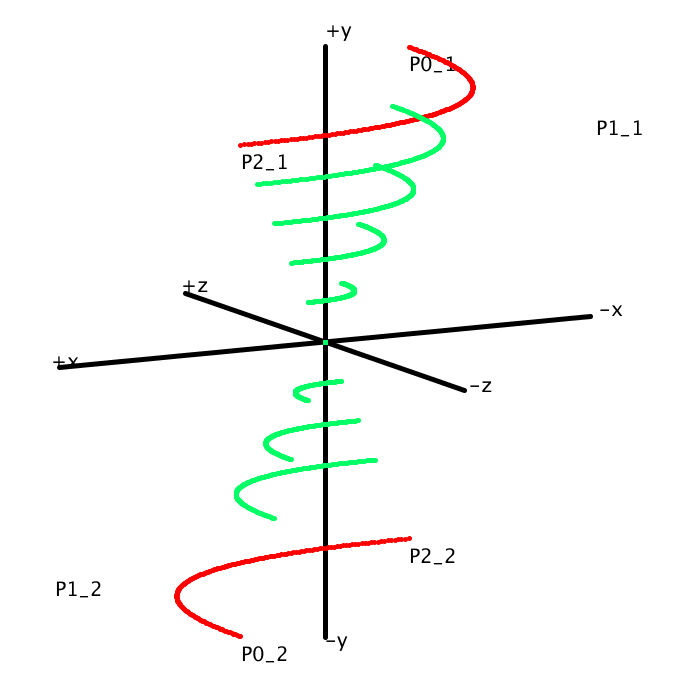
\includegraphics[width=.4\textwidth]{image/BCmovement}
	\caption{베지어 곡선의 움직임}
	\small 처음 곡선과 끝 곡선(빨간색)에 대해 이들을 연속적으로 변화시켜 중간 곡선(초록색)을 만든다.
\end{figure}


다만 이 작업에서 자연스럽게 이동하게 만들어주지만 너무 앞과 끝에 집중되어 맞춰져 있다보니 중간에 원하는 부분이 안 나올 수도 있다. 그것은 움직임이 별로 크지 않도록 프레임을 나눠 사이사이를 다음과 같은 방법을 적용하는 식으로 사용하여 문제를 해결 할 수 있다.
\section{Code Implementation}
\subsection{Lambertian Reflectance} 
프로세싱에서는 명암이 있지 않는다면 단색으로 덮어지는 경향이 있어 3차원 좌표계의 위치를 잘 파악하기 힘들다. 특정한 경우에는 명암을 넣지 않았지만 구의 obj 파일 같이 특정한 파일은 단색에 점들도 아주 많아서 위치를 구별하기 어려웠고 이를 해결하는 것은 필수적이였다. 그래서 많이 사용되는 조명 기법인 Lambertian reflectance를 사용하였다. 이는 실재로 mtl 파일에서 사용되는 기법이다. 

빛의 효과를 받은 물체의 색깔은 전체적으로 3가지 모습의 합쳐진 모습으로 나타난다.
\begin{figure}[h]
	\begin{center}
		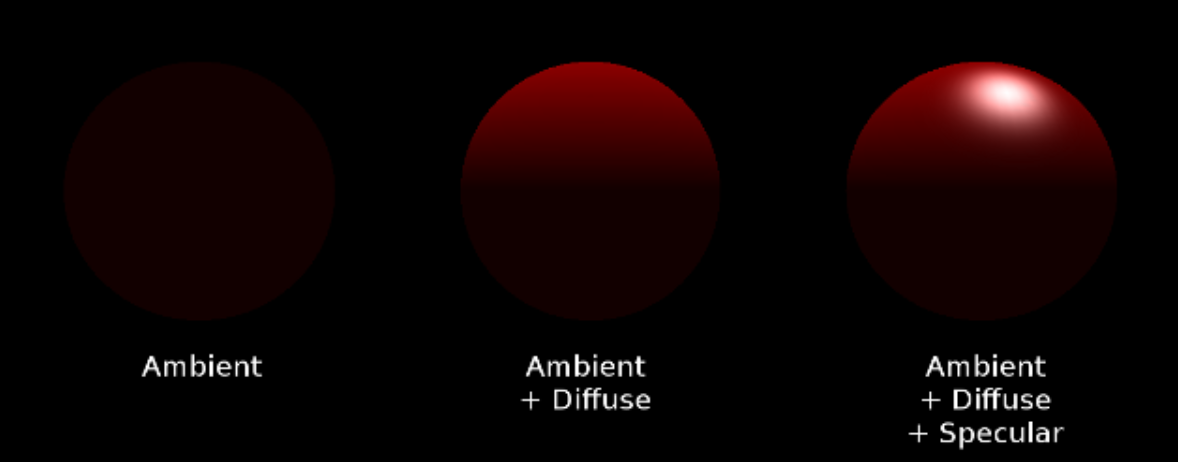
\includegraphics[width=.9\textwidth]{image/lambert3}
	\end{center} \setstretch{1.2}
    \caption{Lambertian reflectance}
	\raggedright \small
	%https://m.blog.naver.com/catllage/220826200078
	ambient color, diffuse color, specular color의 효과를 보여준다. 여기서 ambient color는 평균적인 색상을 의미하는데 전체적으로 어두워 잘 보이지 않지만 잘보면 평균적인 색상을 나타낸다는 것을 알 수 있다.
\end{figure}
\begin{itemize}
	\item 전체적인 평균 색상을 알려주는 ambient 색깔
	\item 물체의 조명의 위치에 따라 부분마다 다른 색깔이 나타날 것이다. 이에 대한 효과는 diffuse 색깔로 나타난다.
	\item 그리고 마지막으로 그 물체의 특수한 재질때문에 생기는 효과로 인한 색깔이 더해진다. 제일 대표적인 예시로 광택이 있으며 이를 specular 색깔이라고 한다.
\end{itemize}
각 ambient 색깔, diffuse 색깔, specular 색깔은 각각 $K_{a}, K_{d}, K_{s}$라 하는 ambient 반사도, diffuse 반사도, specular 반사도에 영향을 받는다. 

이 프로세싱에서 3D 좌표계의 가장 큰 문제는 광택처럼 재질을 표현할수 없는 것이 아니라 부분마다 똑같은 색이 아닌 다른 색이 나타나게 하는 것이다. 그래서 다른 부분은 너무 어려워 다루지 않았고 ambient 반사도, diffuse 반사도 에 해당되는 내용만 다루었다.

이에 대한 식은 다음과 같다.

1. ambient 색깔만 반영하면 최종 색깔은 다음과 같은 식으로 나타난다.
\begin{equation*}
	\begin{split}
		ambient color=material color* ambient 반사도
	\end{split}
\end{equation*}

2. diffuse 색깔까지 반영하면 최종 색깔은 다음과 같은 식으로 나타난다.

\begin{equation*}
	\begin{split}
		&light vector=light position-object position \\
		&cosine=dot product(object normal vector(법선벡터),normalized light vector) \\
		&lambert factor=max(cosine,0) \\
		&luminosity=\frac{1}{1+distance*distance} \\
		&diffuse color=material color*light color*lambert factor* luminosity \\
		&final color=ambient color+diffuse color
	\end{split}
\end{equation*}
이에 대한 부분은 아래 \cref{3D model approximation program}부분에서 확인할 수 있을 것이다.

\subsection{Arc Approximation Program}
이 코드 구현 부분은 2D model improvement 의 알고리즘 부분 \cref{arc_approxiamtion}의 원호 근사 부분 코드이다. 코드 내 함수는 다음과 같다.
\begin{verbatim}
#arc_approximation functions
coordinate3D()
point3D(float x,float y,float z)
point3D_RGB(float x,float y,float z,float R,float G,float B,float st)
line3D_RGB(float x,float y,float z,float w,float m,float n,float R,float G,
float B)
check3D(float x,float y,float z)
Bezier2D(float x0,float y0,float x1,float y1,float x2,float y2,float num)
Bezier3D(float x0,float y0,float z0,float x1,float y1,float z1,float x2,
float y2,float z2, float num)
Bezier_line3D(float x0,float y0,float z0,float x1,float y1,float z1
,float x2,float y2,float z2,float x3,float y3,float z3,float x4,float y4,
float z4,float x5,float y5,float z5)
Bezier_move2D(float x0,float y0,float x1,float y1,float x2,float y2,float x3,
float y3,float x4,float y4,float x5,float y5)
Bezier_move3D(float x0,float y0,float z0,float x1,float y1,float z1,float x2,
float y2,float z2,float x3,float y3,float z3,float x4,float y4,float z4,
float x5,float y5,float z5)
Bezier_move_change3D(float x0,float y0,float z0,float x1,float y1,float z1,
float x2,float y2,float z2,float x3,float y3,float z3,float x4,float y4,
float z4,float x5,float y5,float z5,float k,float R,float G,float B,float m)
circle2D(float r,float n,float start,float last)
makeBezier(float start,float last,float r,float n)
goBezier(float start,float last,float n,float r,float num)
nogoBezier(float start,float last,float n,float r,float num)
noBezier(float x0,float y0,float x1,float y1,float x2,float y2)
Housedorf(float r,float start,float last,float x0,float y0,float x1,float y1,
float x2,float y2,float num)
\end{verbatim}
이것을 프로세싱에 실행시킨뒤 0을 누르면 베지어 곡선이, 1을 누르면 움직이는 베지어 곡선이, 2를 누르면 근사된 결과가 나온다. 근사시킨 것은 2번째줄에서 app라는 근사 기준치를 기준으로 한다. 즉, 여기서 20이라는 것은 오차함수가 20 이하가 되면 멈추게 되는 것이다. 
0,1을 누른상태에서 창을 우클릭하고 움직이면 좌표계가 회전하는 것을 볼 수 있다.
%code%%%%%%%%%%%%%%%%%%%%%%%%%%%%%%%%%%%%%%%%%%%%%%%%%%%%%%%%%%%%%%%%%%%%%%%%%%%%%%%%%%
\begin{multicols}{2}
\lstinputlisting[language=Octave,firstline=1,lastline=163]{curve_approximation/curve_approximation.pde}
\end{multicols}
%%%%%%%%%%%%%%%%%%%%%%%%%%%%%%%%%%%%%%%%%%%%%%%%%%%%%%%%%%%%%%%%%%%%%%%%%%%%%%%%%%%%%%%
\subsection{3D model approximation program} \label{3D model approximation program}
다음은 3D 구면을 근사하는데 필요한 부분 \cref{sphere_approximation} 을 구현한 프로세싱의 java 기반 코드이다. 이외에도 저장형식을 불러오기 위한 컴파일러, 함수 찾는 기능, 파일을 저장하는 기능, 불러오는 기능등을 넣은 것이다. 이 코드만 있으면 되는 것이 아닌 보조 텍스트 파일과 그림파일이 필요하다. 하지만 대략적인 구현 방식만 보여주기 위한 것이고 보조 파일의 내용이 너무 많은 관계로 보조 텍스트 파일의 내용을 쓰지는 않겠다. 

이 코드를 보면 모두 프로세싱의 java 기반 코딩 프로그램에서 한거지만 java, 즉, 객체 지향적 코딩에 익숙하지 않아 벡터 행렬 객체이외에는 c언어 형식으로 써진 것을 확인 할 수 있다. 이를 인지하고 객체 지향적으로 다시 짠다면 랜더링 시간은 물론이고 전반적인 연구의 결과물도 몇배 좋아질 것이라 생각된다.
%code%%%%%%%%%%%%%%%%%%%%%%%%%%%%%%%%%%%%%%%%%%%%%%%%%%%%%%%%%%%%%%%%%%%%%%%%%%%%%%%%%%
\clearpage
\begin{multicols}{2}
	\lstinputlisting[language=Octave,firstline=1,lastline=1991]{sketch_3D_model_approximation_program/sketch_3D_model_approximation_program.pde}
\end{multicols}
%%%%%%%%%%%%%%%%%%%%%%%%%%%%%%%%%%%%%%%%%%%%%%%%%%%%%%%%%%%%%%%%%%%%%%%%%%%%%%%%%%%%%%%
\section{Conclusion}
이 연구에서 임의의 3차원 곡선을 2차 베지어 곡선을 통해 근사할 때에는 3차원 곡선을 조각별로 나누고, 각각의 조각에서 적절한 조절점을 정의하는 방법을 이용함으로써 어떤 곡선이든 충분히 근사 가능함을 알아내었다. 그리고 두 곡선, 즉 처음 곡선과 끝 곡선이 주어졌을 때, 연속적인 변화를 통해 곡선의 움직임을 줄 수 있는 방법을 제시하였다. 

각각의 베지어 곡선을 구성하는데 있어서 세 개의 점의 좌표만이 요구되기 때문에 곡선을 저장하는데 있어서 필요한 용량이 효율적으로 감소된다. 또한 본 연구의 방법을 통해서 3차원 곡선, 곡면을 자유자재로 다룰 수 있기 때문에 VR, 홀로그램 등 미래에 상용화될 것이라고 기대되는 기술들을 구현함에 있어 효과적인 역할을 할수 있을 것이라고 예상된다. 

3D 근사의 경우에는 obj파일로 정점들의 집합과 곡면을 이루는 다각형 면들이 주어졌을 때 베지어 곡면을 이용해 원 곡면을 근사한다. 이를 위해 정점들을 원통형으로 분할하며, 분할된 각 영역에 대해 베지어 곡면의 성질과 Möller–Trumbore intersection algorithm, 최소제곱법, 뉴턴-랩슨 방법을 이용해 베지어 곡면을 구성하는 조절점을 얻는다. 더욱이 제시된 방법에 따라 연구 대상으로 하는 곡면들이 모두 충분히 근사될 수 있음을 보였다. 

실제로 반지름의 길이가 64인 구면에 연구에서 제시한 방법을 적용했을 때, 실행 시간 1분 이내에 오차함수 $\mu<10$을 얻었고 곡면을 저장하는 메모리는 200배 이상 감소 되었다. 

베지어 곡면은 삼각형 분할에 비해 더 효율적이며, 적은 메모리를 요구한다. 그렇기에 본 연구는 VR, AR 등 곡면에 대한 그래픽 기술을 다루는 분야에서의 활용이 기대되며 특히 CAGD 분야에 있어 의미있는 결과이다. 또한 기존에 3D 모델을 저장하기 위해 자주 사용되는 obj파일을 변환시키는 연구이기에 3D 모델링이 필요한 보다 다양한 분야와 접목시킬 수 있다. 

그리고 추가적인 후속연구로 2D,3D 근사 기법을 통해 어떤 색깔 있는 2D,3D 곡면을 더 부드럽게 표현할 수 있었고 모델만 저장하는 형식보다는 아니지만 기존의 RGB 저장 형식을 개선할 수 있었다. 
모델 근사 뿐만 아니라 이에 대한 색깔까지 저장할 수 있으므로 더 많은 쪽에서 활용을 기대할 수 있다.
\clearpage
\begin{thebibliography}{99}\begin{onehalfspace}
    \bibitem{Ji-wung Choi} Ji-wung Choi, Renwick Curry, Babriel Elkaim (2008) “Path Planning Based on Bezier Curve for Autonomous Ground Vehicles”, WCECS 2008.
    \bibitem{Hazewinkel}Hazewinkel, Michiel (1997) “Encyclopaedia of Mathematics: Supplement. 1”, Springer Science \& Business Media, pp. 119.
    \bibitem{Seon-Hong Kim} Seon-Hong Kim, Young Joon Ahn (2007) “Approximation of circular arcs by quartic Bezier ciurves”, Computer-Aided Design 39, pp. 490-493.
    \bibitem{Forrest} A. R. Forrest (1972) “Interactive interpolation and approximation by Bezier polynomials”, The Computer Journal, Vol 15, Issue 1, pp. 71-79.
    \bibitem{Bezier Polynomial} 문성룡, 문홍진, 송의남, 김종교 (1985) “Quadratic Bezier Polynomial 과 B-spline Function을 이용한 Curve Fitting 및 Computer Graphic Animation 에 관한 기초연구”, 대하전자공학회 학술대회, pp. 321-327. 
    \bibitem{Munkres, James} Munkres, James (1999) Topology(2nd ed) Prentice Hall, pp.280-281.
	\bibitem{Farin} Farin, G. E., \& Farin, G. (2002). \emph{Curves and surfaces for CAGD: a practical guide}. Morgan Kaufmann.
	\bibitem{raytriangle} Möller, T., \& Trumbore, B. (1997). Fast, minimum storage ray-triangle intersection. \emph{Journal of graphics tools}, 2(1), 21-28.
	\bibitem{Munkres.J.} Munkres, J. (2014). \emph{Topology}. Pearson Education.
	\bibitem{2021} Lifton, J. J., Liu, T., \& McBride, J. (2021). Non-linear least squares fitting of Bézier surfaces to unstructured point clouds. \emph{AIMS Mathematics}, 6(4), 3142-3159.
\end{onehalfspace}\end{thebibliography}
%   감사의 글
\begin{acknowledgements}
\addcontentsline{toc}{section}{감사의 글}
먼저 지난 3년 동안 저에게 헤아릴 수 없는 많은 가르침을 주신 경기과학고등학교 선생님들께 깊은 감사의 말씀을 올립니다. 항상 부족한 제자였던 저를 넓은 아량으로 감싸주시고 이끌어 주셨기에 제가 이 만큼 성장할 수 있었습니다. 선생님들의 훌륭한 가르침에 마음을 가득 담아 존경을 표하며 감사드립니다. 선생님들의 가르침을 마음 깊이 새기고 앞으로 나아감으로써 은혜에 보답할 수 있도록 하겠습니다. 

기초 R$\&$E와 심화 R$\&$E를 지도해주신 김소연 선생님께도 깊은 감사의 말씀을 올립니다. 2년 동안 연구를 진행하면서 힘들고 어려운 일들이 있을 때마다 많은 조언과 가르침을 주셨기에 연구를 무사히 마무리할 수 있었습니다. 늘 바쁘신 와중에도 이 논문이 처음부터 완성에 이르기까지 물심양면 도와주시고 항상 응원해 주셔서 감사드립니다. 그리고 바쁘신 와중에도 이 논문에 관심을 가져주시고 논문의 심사를 맡아주신 김소연 선생님과 박병철, 서은아 심사위원님께 감사의 말씀을 올립니다.

3년이라는 긴 시간 동안 동고동락한 경기과학고등학교의 선배, 후배, 학우들에게도 감사의 말씀을 드립니다. 선배, 후배, 학우들이 있었기에 힘들 때마다 함께 의지하고 헤쳐나가며 학교생활을 즐겁고 행복하게 할 수 있었습니다. 경기과학고등학교에서 우리가 함께 보낸 소중하고 뜻깊은 고등학교 생활이 앞으로 다가올 제 삶에 훌륭한 밑거름이 될 것이라고 믿습니다. 모두 행복하고 즐거운 삶을 살아가길 진심으로 바라며, 앞으로 하는 모든 일들이 축복과 함께하길 기원합니다.

그리고 사랑하는 가족에게도 감사의 말씀을 올립니다. 가장 힘든 순간마다 언제나 저를 지지해 주시고 격려해주신 부모님께 감사드립니다. 항상 저에 대해 함께 고민해 주시고 지혜 담긴 말씀들로 저의 갈 길을 열어주신 부모님과 동생인 저를 아끼고 지지해 준 누나에게 진심어린 사랑을 전합니다. 

지금까지 너무나 많은 분들이 저에게 큰 도움을 주셨기에 이 짧은 감사의 글로 제 마음을 다 표현할 수는 없지만, 지금까지 함께 해주신 모든 분들께 진심으로 감사의 말씀을 올리며, 저에게 보내주신 응원과 사랑을 마음 깊이 새기고 앞으로도 최선을 다하는 삶을 살아가겠습니다. 감사합니다.
\end{acknowledgements}
%   연구활동 
\begin{researches}
\addcontentsline{toc}{section}{연구활동}
\begin{itemize}
\item{2020 국제수학교육학술대회 R$\&$E 포스터 논문 발표 대회 장려상 수상}
\item{2021 심화 R$\&$E 우수상(수학 부문)}
\item{2021 영재학교 우수 R$\&$E 공동발표회 우수상}
\item{2021 삼성휴먼테크논문대상 (수학/전산부문) 동상}
\end{itemize}
\end{researches}
\end{document} 
